\documentclass[a4paper,12pt,twoside]{memoir}

% Castellano
\usepackage[spanish,es-tabla]{babel}
\selectlanguage{spanish}
\usepackage[utf8]{inputenc}
\usepackage[T1]{fontenc}
\usepackage{lmodern} % Scalable font
\usepackage{microtype}
\usepackage{placeins}

\RequirePackage{booktabs}
\RequirePackage[table]{xcolor}
\RequirePackage{xtab}
\RequirePackage{multirow}

% Links
\usepackage[colorlinks]{hyperref}
\hypersetup{
	allcolors = {red}
}

% Ecuaciones
\usepackage{amsmath}

% Rutas de fichero / paquete
\newcommand{\ruta}[1]{{\sffamily #1}}

% Párrafos
\nonzeroparskip


% Imagenes
\usepackage{graphicx}
\newcommand{\imagen}[2]{
	\begin{figure}[!h]
		\centering
		\includegraphics[width=0.9\textwidth]{#1}
		\caption{#2}\label{fig:#1}
	\end{figure}
	\FloatBarrier
}

\newcommand{\imagenflotante}[2]{
	\begin{figure}%[!h]
		\centering
		\includegraphics[width=0.9\textwidth]{#1}
		\caption{#2}\label{fig:#1}
	\end{figure}
}

\usepackage{dirtree}

\usepackage{listings}
\lstset{basicstyle=\normalfont\ttfamily,
	showstringspaces=false,
	commentstyle=\color{gray},
	keywordstyle=\color{magenta!60!black},
	breaklines=true,
	resetmargins=true
}

\usepackage{pdfpages}

\widowpenalty10000
\clubpenalty10000

% El comando \figura nos permite insertar figuras comodamente, y utilizando
% siempre el mismo formato. Los parametros son:
% 1 -> Porcentaje del ancho de página que ocupará la figura (de 0 a 1)
% 2 --> Fichero de la imagen
% 3 --> Texto a pie de imagen
% 4 --> Etiqueta (label) para referencias
% 5 --> Opciones que queramos pasarle al \includegraphics
% 6 --> Opciones de posicionamiento a pasarle a \begin{figure}
\newcommand{\figuraConPosicion}[6]{%
  \setlength{\anchoFloat}{#1\textwidth}%
  \addtolength{\anchoFloat}{-4\fboxsep}%
  \setlength{\anchoFigura}{\anchoFloat}%
  \begin{figure}[#6]
    \begin{center}%
      \Ovalbox{%
        \begin{minipage}{\anchoFloat}%
          \begin{center}%
            \includegraphics[width=\anchoFigura,#5]{#2}%
            \caption{#3}%
            \label{#4}%
          \end{center}%
        \end{minipage}
      }%
    \end{center}%
  \end{figure}%
}

%
% Comando para incluir imágenes en formato apaisado (sin marco).
\newcommand{\figuraApaisadaSinMarco}[5]{%
  \begin{figure}%
    \begin{center}%
    \includegraphics[angle=90,height=#1\textheight,#5]{#2}%
    \caption{#3}%
    \label{#4}%
    \end{center}%
  \end{figure}%
}
% Para las tablas
\newcommand{\otoprule}{\midrule [\heavyrulewidth]}
%
% Nuevo comando para tablas pequeñas (menos de una página).
\newcommand{\tablaSmall}[5]{%
 \begin{table}
  \begin{center}
   \rowcolors {2}{gray!35}{}
   \begin{tabular}{#2}
    \toprule
    #4
    \otoprule
    #5
    \bottomrule
   \end{tabular}
   \caption{#1}
   \label{tabla:#3}
  \end{center}
 \end{table}
}

%
% Nuevo comando para tablas pequeñas (menos de una página).
\newcommand{\tablaSmallSinColores}[5]{%
 \begin{table}[H]
  \begin{center}
   \begin{tabular}{#2}
    \toprule
    #4
    \otoprule
    #5
    \bottomrule
   \end{tabular}
   \caption{#1}
   \label{tabla:#3}
  \end{center}
 \end{table}
}

\newcommand{\tablaApaisadaSmall}[5]{%
\begin{landscape}
  \begin{table}
   \begin{center}
    \rowcolors {2}{gray!35}{}
    \begin{tabular}{#2}
     \toprule
     #4
     \otoprule
     #5
     \bottomrule
    \end{tabular}
    \caption{#1}
    \label{tabla:#3}
   \end{center}
  \end{table}
\end{landscape}
}

%
% Nuevo comando para tablas grandes con cabecera y filas alternas coloreadas en gris.
\newcommand{\tabla}[6]{%
  \begin{center}
    \tablefirsthead{
      \toprule
      #5
      \otoprule
    }
    \tablehead{
      \multicolumn{#3}{l}{\small\sl continúa desde la página anterior}\\
      \toprule
      #5
      \otoprule
    }
    \tabletail{
      \hline
      \multicolumn{#3}{r}{\small\sl continúa en la página siguiente}\\
    }
    \tablelasttail{
      \hline
    }
    \bottomcaption{#1}
    \rowcolors {2}{gray!35}{}
    \begin{xtabular}{#2}
      #6
      \bottomrule
    \end{xtabular}
    \label{tabla:#4}
  \end{center}
}

%
% Nuevo comando para tablas grandes con cabecera.
\newcommand{\tablaSinColores}[6]{%
  \begin{center}
    \tablefirsthead{
      \toprule
      #5
      \otoprule
    }
    \tablehead{
      \multicolumn{#3}{l}{\small\sl continúa desde la página anterior}\\
      \toprule
      #5
      \otoprule
    }
    \tabletail{
      \hline
      \multicolumn{#3}{r}{\small\sl continúa en la página siguiente}\\
    }
    \tablelasttail{
      \hline
    }
    \bottomcaption{#1}
    \begin{xtabular}{#2}
      #6
      \bottomrule
    \end{xtabular}
    \label{tabla:#4}
  \end{center}
}

%
% Nuevo comando para tablas grandes sin cabecera.
\newcommand{\tablaSinCabecera}[5]{%
  \begin{center}
    \tablefirsthead{
      \toprule
    }
    \tablehead{
      \multicolumn{#3}{l}{\small\sl continúa desde la página anterior}\\
      \hline
    }
    \tabletail{
      \hline
      \multicolumn{#3}{r}{\small\sl continúa en la página siguiente}\\
    }
    \tablelasttail{
      \hline
    }
    \bottomcaption{#1}
  \begin{xtabular}{#2}
    #5
   \bottomrule
  \end{xtabular}
  \label{tabla:#4}
  \end{center}
}



\definecolor{cgoLight}{HTML}{EEEEEE}
\definecolor{cgoExtralight}{HTML}{FFFFFF}

%
% Nuevo comando para tablas grandes sin cabecera.
\newcommand{\tablaSinCabeceraConBandas}[5]{%
  \begin{center}
    \tablefirsthead{
      \toprule
    }
    \tablehead{
      \multicolumn{#3}{l}{\small\sl continúa desde la página anterior}\\
      \hline
    }
    \tabletail{
      \hline
      \multicolumn{#3}{r}{\small\sl continúa en la página siguiente}\\
    }
    \tablelasttail{
      \hline
    }
    \bottomcaption{#1}
    \rowcolors[]{1}{cgoExtralight}{cgoLight}

  \begin{xtabular}{#2}
    #5
   \bottomrule
  \end{xtabular}
  \label{tabla:#4}
  \end{center}
}


















\graphicspath{ {./img/} }

% Capítulos
\chapterstyle{bianchi}
\newcommand{\capitulo}[2]{
	\setcounter{chapter}{#1}
	\setcounter{section}{0}
	\chapter*{#2}
	\addcontentsline{toc}{chapter}{#2}
	\markboth{#2}{#2}
}

% Apéndices
\renewcommand{\appendixname}{Apéndice}
\renewcommand*\cftappendixname{\appendixname}

\newcommand{\apendice}[1]{
	%\renewcommand{\thechapter}{A}
	\chapter{#1}
}

\renewcommand*\cftappendixname{\appendixname\ }

% Formato de portada
\makeatletter
\usepackage{xcolor}
\newcommand{\tutor}[1]{\def\@tutor{#1}}
\newcommand{\course}[1]{\def\@course{#1}}
\definecolor{cpardoBox}{HTML}{E6E6FF}
\def\maketitle{
  \null
  \thispagestyle{empty}
  % Cabecera ----------------
\noindent
\includegraphics[width=\textwidth]{cabecera}\vspace{1cm}%
  \vfill
  % Título proyecto y escudo informática ----------------
  \colorbox{cpardoBox}{%
    \begin{minipage}{.8\textwidth}
      \vspace{.5cm}\Large
      \begin{center}
      \textbf{TFG del Grado en Ingeniería Informática}\vspace{.6cm}\\
      \textbf{\LARGE\@title{}}
      \end{center}
      \vspace{.2cm}
    \end{minipage}

  }%
  \hfill\begin{minipage}{.20\textwidth}
    
\includegraphics[width=\textwidth]{escudoInfor}
  \end{minipage}
  \vfill
  % Datos de alumno, curso y tutores ------------------
  \begin{center}%
  {%
    \noindent\LARGE
    Presentado por \@author{}\\ 
    en Universidad de Burgos --- \@date{}\\
    Tutores: \@tutor{}\\
  }%
  \end{center}%
  \null
  \cleardoublepage
  }
\makeatother

\newcommand{\nombre}{José Miguel Ramírez Sanz} %%% cambio de comando

% Datos de portada
\title{AVC \\ Asistente Virtual para la Comunicación}
\author{\nombre}
\tutor{Dr. José Francisco Díez Pastor y Dr. César Represa Pérez}
\date{\today}

\begin{document}

\maketitle


\newpage\null\thispagestyle{empty}\newpage


%%%%%%%%%%%%%%%%%%%%%%%%%%%%%%%%%%%%%%%%%%%%%%%%%%%%%%%%%%%%%%%%%%%%%%%%%%%%%%%%%%%%%%%%
\thispagestyle{empty}


\noindent
\includegraphics[width=\textwidth]{cabecera}\vspace{1cm}

\noindent Dr. D. José Francisco Díez Pastor, profesor del departamento de Ingeniería Civil, área de Lenguajes y Sistemas Informáticos y Dr. D. César Represa Pérez, profesor del departamento de Ingeniería Electromecánica, área de Tecnología Electrónica.

\noindent Exponen:

\noindent Que el alumno D. \nombre, con DNI 71303106R, ha realizado el Trabajo final de Grado en Ingeniería Informática titulado \textit{AVC Asistente Virtual para la Comunicación}. 

\noindent Y que dicho trabajo ha sido realizado por el alumno bajo la dirección del que suscribe, en virtud de lo cual se autoriza su presentación y defensa.

\begin{center} %\large
En Burgos, {\large \today}
\end{center}

\vfill\vfill\vfill

% Author and supervisor
\begin{minipage}{0.45\textwidth}
\begin{flushleft} %\large
Vº. Bº. del Tutor:\\[2cm]
Dr. D. José Francisco Díez Pastor
\end{flushleft}
\end{minipage}
\hfill
\begin{minipage}{0.45\textwidth}
\begin{flushleft} %\large
Vº. Bº. del co-tutor:\\[2cm]
Dr. D. César Represa Pérez	
\end{flushleft}
\end{minipage}
\hfill

\vfill

% para casos con solo un tutor comentar lo anterior
% y descomentar lo siguiente
%Vº. Bº. del Tutor:\\[2cm]
%D. nombre tutor


\newpage\null\thispagestyle{empty}\newpage




\frontmatter

% Abstract en castellano
\renewcommand*\abstractname{Resumen}
\begin{abstract}
La parálisis cerebral es una discapacidad que afecta a la capacidad de movimiento y de la postura. Además, esta discapacidad suele ir acompañada de otras discapacidades en la percepción de los sentidos y en la capacidad cognitiva. Dentro de las personas afectas hay un grupo gravemente afectado con grandes discapacidades motoras, cognitivas y sobre todo comunicativas, ya que los únicos sonidos que emiten son ruidos.

Con la idea de facilitar la comunicación de estos pacientes gravemente afectados surgió la propuesta desde APACE Burgos para desarrollar un comunicador virtual con el que poder interpretar los sonidos que estas personas hacen. Es aquí cuando APACE Burgos se puso en contacto con la Universidad de Burgos para desarrollar AVC, el \textit{Asistente Virtual para la Comunicación}.

Para la realización de este proyecto se han desarrollado varias aplicaciones. Una para la recogida de los sonidos procedentes de los pacientes con los que entrenar un clasificador, y otra aplicación para la interpretación de los sonidos emitidos por los pacientes en base a los datos registrados. También se ha desarrollado un servidor que permite el almacenamiento de las opciones adicionales necesarias para la clasificación, así como para poder interpretar los sonidos.

Las aplicaciones generadas durante este proyecto se han desarrollado en \textit{Android} y se ha usado \textit{Python} para desarrollar el servidor. El asistente pretende reconocer emociones (hambre, tristeza, enfado y dolor) y respuestas (sí y no) a partir de métodos de clasificación. Para ello se han empleado algoritmos de extracción de características sobre audios, y para el clasificador final se ha usado un tipo de \textit{ensemble} llamado \textit{Bagging}, en concreto \textit{Random Forest}.
\end{abstract}

\renewcommand*\abstractname{Descriptores}
\begin{abstract}
Parálisis cerebral, comunicación, extracción de características, clasificación de audios, \textit{Random Forest}, \textit{Android}, servidor \textit{Flask}.
\end{abstract}

\clearpage

% Abstract en inglés
\renewcommand*\abstractname{Abstract}
\begin{abstract}
Cerebral palsy is a disability that affects the ability to move and posture. Besides, this disability is often accompanied by other diabilities in the senses and the cognitive ability. There is a group of people severely affected with large motor, cognitive and, above all, communicative disabilities, because they can only communicate by noises.

Thinking about facilating communication to severely affected patients, APACE Burgos suggested to develop a virtual communicator to interpret the sounds of these people. Here is when APACE Burgos contacted with University of Burgos to develop VCA, the \textit{Virtual Assitant for Communication}.

For the realization of this project they have been developed some applications. One for collectiong data from patients, and other one to interpret the sounds emitted by patients. A server has also been developed, to allow storage of the necesaary additional options for the classification.

The generated applications during this project have been developed in \textit{Android} and we have used \textit{Python} for the development of the server. To design the algorithms of classification of emotions (hungry, sadness, anger and pain) and answers (yes and no) feature extraction algorithms on sounds has been used, and for the final classifier we have applied a type of ensemble called \textit{Bagging}, specifically \textit{Random Forest}.
\end{abstract}

\renewcommand*\abstractname{Keywords}
\begin{abstract}
Cerebral palsy, communication, feauture extraction, sound classification, \textit{Random Forest}, \textit{Flask} server.
\end{abstract}

\clearpage

% Indices
\tableofcontents

\clearpage

\listoffigures

\clearpage

\listoftables
\clearpage

\mainmatter
\capitulo{1}{Introducción}

La \textbf{parálisis cerebral} es una discapacidad, normalmente originada en la fase de gestación del feto, que afecta al sistema motor de la persona, causando problemas en los movimientos y la postura. Esta discapacidad o conjunto de trastornos son \textbf{permanentes y no progresivos}. A menudo, estas personas padecen otro tipo de discapacidades. Estas suelen afectar al sistema nervioso causando limitaciones en la capacidad de usar los sentidos con los cuales percibir los estímulos exteriores y limitaciones en la capacidad intelectual. Por ello, a la parálisis cerebral se le puede llamar una pluridiscapacidad. \cite{aspacequees,aspacecyl,rosenbaum2007report}

Este conjunto de \textbf{discapacidades} producen una gran limitación en las tareas que las personas que lo sufren pueden realizar. Al ser parte de las discapacidades relacionadas con la postura y el sistema motor del cuerpo, las carencias en cuanto al movimiento son claras. Además, las discapacidades en el sistema nerviosos que pueden causar limitaciones sensoriales y cognitivas que pueden llevar a restricciones en la percepción del mundo exterior, en la conducta o en la \textbf{comunicación}.

La parálisis cerebral se origina principalmente en la gestación del feto y es causada por tres tipos de factores: \textbf{prenatales} causados por alteraciones en la coagulación o de la placenta, por traumatismos, por infecciones y por otras causas incluida la gestación múltiple, \textbf{perinatales} donde nos encontramos con diferentes causas entre las que destaca la prematuridad y por último, \textbf{postnatales}, a partir de más de 28 días después del nacimiento, donde encontramos causas como traumatismos craneales postnatales, paradas cardio-respiratorias, etc.\cite{crene,causas}

Como ya se ha comentado antes, la parálisis cerebral es una discapacidad que afecta a un gran número de personas, pero cada parálisis cerebral es diferente. Según ASPACE, 1 de cada 500 personas nacen en España con parálisis cerebral, lo que nos lleva a un total de 120.000 personas en todo el país.\cite{aspacedatos}

Hay distintos tipos, e incluso de clasificaciones, de parálisis cerebral. En el extremo de las personas más afectadas nos encontramos con las mayores carencias que he comentado, estas personas sufren de una gran limitación de movimiento y postura. Tienen que estar todo el día en una cama y si se quieren mover, montados en sillas especiales hechas a medida para no producirles ningún tipo de molestia ni de lesión. Uno de los mayores problemas que tienen las personas que padecen este grado de discapacidad es la limitación en la \textbf{comunicación}, ya que debido a sus carencias en la capacidad de moverse y de controlar estos movimientos solo pueden emitir \textbf{ruidos} o carcajadas, y en algunos casos ni siquiera se puede saber si tienen una intención comunicativa, es decir, emiten esos ruidos para intentar comunicarse, o simplemente son ruidos sin sentido.

Hoy en día se usan distintas aplicaciones y programas para que personas con parálisis cerebral se puedan comunicar \cite{jocomunico}, pero estas aplicaciones no pueden ser usadas por las personas gravemente afectadas debido a sus restricciones en el movimiento y control de su cuerpo. Esto es un gran problema ya que les excluye de usar estas herramientas para poder comunicarse. Como he comentado anteriormente, las personas gravemente afectadas solo emiten ruidos, los cuales pueden o no tener una intención comunicativa. Solo los familiares y los cuidadores más cercanos a la persona pueden llegar a intuir si ese ruido tiene alguna intención y, si la tiene, poder interpretarlo para saber si, por ejemplo, tiene hambre o le duele algo. El problema está en si esta persona con parálisis cerebral se tiene que quedar, por ejemplo, con un cuidador nuevo que no conoce ni puede interpretar estos sonidos.

Es por ello que comenzó el desarrollo de \textbf{AVC}, una aplicación Android accesible e intuitiva, que nos permite interpretar la emoción o la respuesta de una persona con parálisis cerebral gravemente afectada a partir de los sonidos que emite, gracias a métodos de clasificación de minería de datos.

\section{Estructura de la Memoria}
La presente memoria se compone de los siguiente apartados: 
\begin{itemize}
	\item 
		\textbf{Introducción:} descripción de la parálisis cerebral, planteamiento del problemas e introducción de la solución.
	\item
		\textbf{Objetivos del proyecto:} conjunto de objetivos funcionales, técnicos y personales que se han tenido a lo largo de este proyecto.
	\item
		\textbf{Conceptos teóricos:} explicación de nociones teóricas básicas para poder entender el proyecto.
	\item
		\textbf{Técnicas y herramientas:} conjunto de técnicas y herramientas esenciales en el desarrollo del proyecto.
	\item
		\textbf{Aspectos relevantes del desarrollo:} explicación temporal de los hechos más relevantes del proyecto.
	\item
		\textbf{Trabajos relacionados:} herramientas y proyectos semejantes.
	\item
		\textbf{Conclusiones:} conclusiones sobre el desarrollo del proyecto y posibles líneas futuras de trabajo.
\end{itemize}

\section{Estructura de los Anexos}
El documento con los anexos tiene los siguiente componentes:
\begin{itemize}
	\item
	\textbf{Plan del proyecto:} planificación temporal y viabilidad económica y legal del proyecto.
	\item
	\textbf{Requisitos:} diseño de los casos de usos, y de los requisitos funcionales y no funcionales.
	\item
	\textbf{Diseño:} explicación de las distintas fases de diseño seguidas en la aplicación.
	\item
	\textbf{Manual del programador:} manual por el cual un desarrollador podría poner en funcionamiento los elementos del proyectos o proseguir su implementación.
	\item
	\textbf{Manual de usuario:} conjunto de manual para la correcta instalación y ejecución de las aplicaciones desarrolladas en el proyecto.
\end{itemize}

\section{Materiales adjuntos}
Los elementos desarrollados y documentados durante el proyecto se pueden ver en el repositorio en \textit{GitHub}, \url{https://github.com/Josemi/AVC-TFG}.
Junto con esta memoria se entrega un CD con el siguiente contenido:
\begin{itemize}
	\item Memoria en formato pdf.
	\item Anexos en formato pdf.
	\item Aplicación para la recogida de datos, prototipo inicial.
	\item Aplicación para la recogida de datos, versión final.
	\item Aplicación AVC para poder interpretar los sonidos de las personas con las que se ha entrenado.
	\item Servidor en Flask para la administración de los datos y para el procesamiento y clasificación de los audios.
	\item Documentación \textit{javadoc}, de las tres aplicaciones \textit{Android}.
	\item Manuales de usuario para las tres aplicaciones.
	\item Presentaciones de las aplicaciones que se han usado para enseñar el proyecto en diversas situaciones.
	\item Vídeos e imágenes de las diversas presentaciones que se han realizado en el proyecto.
\end{itemize}	
\capitulo{2}{Objetivos del proyecto}

En este apartado voy a comentar los distintos objetivos funcionales, técnicos y personales del proyecto.

\section{Objetivos funcionales}
En este subapartado voy a contar cuales han sido los objetivos, en cuanto a qué queríamos que hiciesen las distintas aplicaciones del proyecto.
\begin{itemize}
	\item
	Tener una aplicación Android que nos permita recoger los audios y las opciones adicionales de cada paciente y poder subirlos para su posterior tratado y análisis, con la finalidad de encontrar el mejor algoritmo de clasificación posible para la aplicación final.
	\item
	Realizar una aplicación Android para la interpretación de los audios. En la aplicación se tiene que poder modificar las opciones adicionales de los pacientes, almacenándose en el servidor para no tener que ponerlas en cada ejecución.
	\item
	Hacer que ambas aplicaciones sean simples de usar y con una ejecución muy lineal.
	\item
	Diseñar una aplicación que sea accesible para que pueda ser usada hasta por compañeros con parálisis cerebral u otro tipo de discapacidad.
	\item
	Dar difusión mediática del proyecto a través de la grabación vídeos, haciendo presentaciones, etc.
\end{itemize}

\section{Objetivos técnicos}
Los objetivos técnicos son los que he tenido en cuenta a lo largo del desarrollo en cuanto a las herramientas y el uso de éstas.
\begin{itemize}
	\item
	Generar dos aplicaciones, la de obtención de datos y la de interpretación de sonidos, que tengan una versión de API mínima de 23 (a partir de Android 6.0), para poder abarcar un mayor número de dispositivos donde se puedan usar.
	\item 
	Utilizar \textit{Python} para la clasificación, por el conocimiento que ya tengo y por el uso de librerías avanzadas en métodos de clasificación como puede ser \textit{Scikit-Learn}.
	\item
	Usar \textit{Flask} como \textit{framework} para el servidor.
	\item 
	Usar un repositorio \textit{Git} para tener un seguimiento del desarrollo y un control de versiones usando \textit{GitHub}.
	\item 
	Usar \textit{ZenHub} para controlar las tareas y tiempos del proyecto.
	\item
	Realizar pruebas unitarias y de integración sobre la aplicación final.
	\item
	Realizar el desarrollo del proyecto siguiendo el modelo \textit{SCRUM}, orientado al trabajo individua, sobre todo en la filosofía incremental de los productos.
\end{itemize}

\section{Objetivos personales}\label{objpers}
En este apartado quiero comentar los objetivos propios que he tenido con este proyecto.
\begin{itemize}
	\item
	Poder ayudar a personas con parálisis cerebral.
	\item 
	Mejorar mi capacidad de comunicación y exposición, preparando diversas presentaciones.
	\item
	Usar el conocimiento obtenido a lo largo de la carrera.
	\item 
	Aprender a programar en Android, ya que es uno de los sistemas operativos más importantes a día de hoy.
	\item 
	Aprender a desarrollar y desplegar un servidor.
	\item 
	Aprender a usar nuevas herramientas de documentación, como \LaTeX.
	\item 
	Aprender a usar nuevas herramientas de diseño y programación.
\end{itemize}
\capitulo{3}{Conceptos teóricos}

En este apartado voy a comentar los distintos conceptos teóricos del proyecto, que van desde la parálisis cerebral hasta conceptos como \textit{Random Forest}.

\section{Parálisis Cerebral}
Como ya he comentado, la parálisis cerebral es un discapacidad en el sistema motor y en la postura de la persona. Además, esta discapacidad suele ir acompañada de otras discapacidades en el sistema nervioso que producen limitaciones en los sentidos y en la capacidad cognitiva de la persona~\cite{rosenbaum2007report,aspacecyl}.

El origen de esta discapacidad se debe a varios factores, mayoritariamente relacionados con el desarrollo del feto. Además, el grado de afección de la parálisis cerebral es distinto en cada caso, teniendo desde personas levemente afectadas que solo sufren de una discapacidad motora, hasta personas gravemente afectadas con grandes discapacidades motoras, cognitiva, sensoriales...

Existen diversas asociaciones que ayudan a las personas que tienen parálisis cerebral y a las familias, amigos o cualquier persona que acompañe a la persona afectada. Por suerte, en España existen multitud de estas asociaciones, siendo Confederación ASPACE~\cite{aspace} la confederación a nivel nacional. En Castilla y León la asociación es ASPACE Castilla y León, y en Burgos tenemos a APACE Burgos~\ref{fig:apace}~\cite{apace}.
\begin{figure}
	\centering
	
\includegraphics[width=\textwidth]{apace}
	\caption{Logotipo de APACE Burgos a la izquierda y ASPACE CyL a la derecha.}
	\label{fig:apace}
\end{figure}
\section{Señal de audio}
El asistente desarrollado toma como entrada un audio y un conjunto de opciones adicionales que hemos obtenido en colaboración con APACE.
\subsection{Sonido}
Una señal sonora es una  perturbación mecánica (vibraciones) en la presión del aire \cite{pierce1995senales}. Ésta se convierte a una señal eléctrica, en concreto a una señal analógica, que es una señal generada por un fenómeno electromagnético que se puede representar a través de una función continua cuyos parámetros son la amplitud y el periodo \cite{analogica}, mediante un proceso electromagnético. Posteriormente es digitalizada a través de un proceso de muestreo, determinado por la frecuencia de muestreo o \textit{sampling rate}, y de un proceso de cuantificación, que junto con la frecuencia de muestreo determina el \textit{bitrate} de la señal digital. A esta señal almacenada se le llama señal de audio, y esta puede ser obviamente almacenada, reproducida y modificada.
\subsection{Espectrograma}
Es una representación gráfica de las señales de audio, es decir, una representación de las frecuencias de la señal sonora almacenada en la señal analógica que compone la señal de audio~\cite{wiki:espec}. En esta representación la distribución de energía se muestra en tres ejes, siendo el eje de las \textit{x} el eje temporal, el eje de las \textit{y} el de las frecuencias y el color (como eje z) muestra el dominio o la distribución de la señal de audio con respecto a los otros dos ejes, el tiempo y las frecuencias~\cite{granesp}.

Como ya comenté, las señales de audio se caracterizan por su periodo y amplitud, como se puede ver en la representación de la onda en la figura~\ref{fig:onda}. En cambio, el espectrograma de éste se muestra en la figura~\ref{fig:espec} en una escala lineal, y en una escala logarítmica en la figura~\ref{fig:especlog}.
\begin{figure}
	\centering
	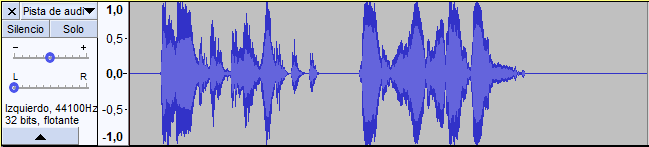
\includegraphics[width=\textwidth]{onda}
	\caption{Representación de la onda. En el eje \textit{x} se representa el tiempo y en el eje \textit{y} la amplitud.}
	\label{fig:onda}
\end{figure}
\begin{figure}
	\centering
	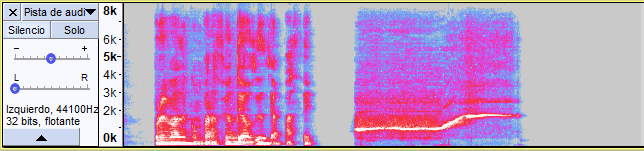
\includegraphics[width=\textwidth]{especlineal}
	\caption{Espectrograma en escala lineal. En el eje \textit{x} se representa el tiempo y en el eje \textit{y} la componente espectral (frecuencia) en escala lineal.}
	\label{fig:espec}
\end{figure}
\begin{figure}
	\centering
	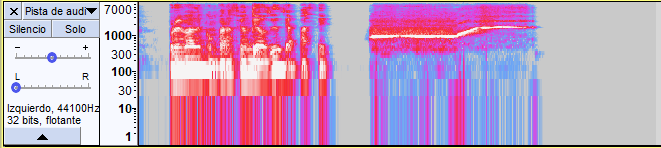
\includegraphics[width=\textwidth]{especlog}
	\caption{Espectrograma en escala logarítmica. En el eje \textit{x} se representa el tiempo y en el eje \textit{y} la componente espectral (frecuencia) en escala logarítmica.}
	\label{fig:especlog}
\end{figure}
\subsection{Frecuencias en escala de Mel, MFCC} \label{mel}
Es una escala que surgió con el objetivo de obtener una escala orientada al sistema auditivo del ser humano, lo que se llama una escala psicoacústica. Su finalidad es poder extraer características de la señal de audio para obtener información. Podemos ver el ejemplo del mismo audio en la figura~\ref{fig:mel}

Esta es la fórmula de las frecuencias en escala de Mel y las frecuencias en escala lineal (f)\cite{wiki:mel,villa2012automatic}: \[ Mel(f) = 2595 * \log_{10}(1+\frac{f}{700})\]

MFCC (\textit{Coeficientes Cepstrales en las Frecuencias de Mel}) son los coeficientes necesarios para esta representación del sonido relacionado con el sistema auditivo humano. El proceso de obtención de este coeficiente sigue los siguientes pasos~\cite{wiki:mel,yeo2011animal}:
\begin{itemize}
	\item División del audio en fragmentos (\textit{frames}).
	\item Minimizar las discontinuidades de la señal en el comienzo y final de cada fragmento.
	\item Aplicar la Transformada Discreta de \textit{Fourier} para conseguir la potencia espectral.
	\item Aplicar los filtros correspondientes a la escala de \textit{Mel}.
	\item De cada frecuencia de \textit{Mel} de las energías obtenemos el logaritmo.
	\item Aplicamos la transformada de coseno discreta a los logaritmos.
\end{itemize}
\begin{figure}
	\centering
	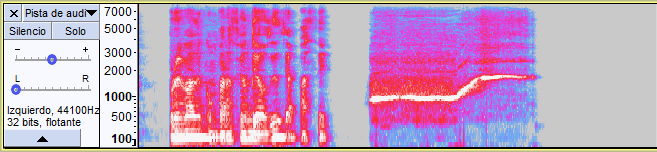
\includegraphics[width=\textwidth]{mel}
	\caption{Espectrograma en escala de Mel. En el eje \textit{x} se representa el tiempo, en el eje \textit{y} las frecuencias relativas a la capacidad auditiva humana.}
	\label{fig:mel}
\end{figure}

\subsection{Zero Crossing Rate} \label{zcr}
Es el ratio que mide el número de veces en las cuales la señal cambia de signo.
\subsection{Bitrate}
Es la unidad de datos que se recogen por unidad de tiempo. Los datos recogidos se miden en bits, mientras que el tiempo se mide en segundos.
Cuando trabajamos con sistemas de recogida de datos, en nuestro caso grabaciones de audios, el \textit{bitrate} de esta recogida es un valor muy importante, ya que determina la cantidad de datos que vamos a obtener. Esta medida puede ser muy interesante a la par de necesaria ya que, junto con el formato y el códec, va a determinar cuánto ocupan los archivos que obtenemos además de la calidad de estos.
\subsection{Sampling Rate}
El Sampling Rate o frecuencia de muestreo es la tasa que marca la cantidad de muestras que se hacen por unidad de tiempo. Partiendo de nuestra función continua, que es la señal analógica, que recoge la señal sonora, es decir, la señal de audio, pasamos a valores discretos. La unidad con la que se mide es, como en todas las frecuencias, $s^{-1}$ o \textit{Hz}~\cite{wiki:sampling}.

\subsection{Formato digital}
Dentro de una señal de audio, y en general para cualquier tipo de dato que se almacena de forma digital, el formato es el estándar, con el cual el dato se codifica, se decodifica y se lee.

Dentro de los formatos que existen en las señales de audios o formatos contenedores de audios podemos diferenciarlos entre los que tienen pérdida de información o \textit{Lossy} y los que no la tienen o \textit{Loseless}. Los formatos que tienen pérdida suelen ser formatos más ligeros, en los cuales los ficheros ocupan menos y son más fáciles de procesar. En cambio, como su nombre indica, tienen pérdidas de información~\cite{wiki:formatoaudio}. 
\subsection{Encoder}
El encoder o códec son los métodos por los cuales podemos codificar y decodificar los datos de audios almacenados en el formato seleccionado. Para cada códec disponemos de una serie de formatos en los cuales se puede codificar y decodificar, por lo que en si, la combinación códec-formato es la que puede ser \textit{Lossy} o \textit{Loseless}~\cite{wiki:codec}.

La mayoría de códecs son  \textit{Lossy}, es decir, pierden información en la codificación que luego no se puede recuperar en la decodificación, alguno de los códecs de audios más usados son los que se pueden observar en la tabla~\ref{tabla:codecaudio}.
\tablaSmall{Códecs de audio}{l c c}{codecaudio}
{ \multicolumn{1}{l}{\textbf{Códecs}} & \textbf{\textit{Lossy}} & \textbf{\textit{Loseless}} \\}{ 
	AAC-LC & X &\\
	AAC-ELD & X &\\
	HE-AAC & X &\\
	AMR-NB & X &\\
	AMR-WB & X &\\
	PCM(Pulse Code Modulations) & & X\\
	FLAC & & X\\
} 
\subsection{Base64}
Método que nos permite codificar cualquier tipo de dato y/o archivo en texto ASCII y decodificarlo. Este tipo de codificación no es la más eficiente que existe, pero si que nos puede servir si queremos mandar nuestros ficheros en modo texto, como pasa en este proyecto, donde tenemos que enviar el audio grabado al servidor a través de un método post donde las variables se pasan en la URL.
\subsection{Extracción de características}
Proceso por el cual podemos obtener información a partir de datos. Se suele llevar a cabo en el preprocesado de información de entrada de los métodos de clasificación de minería de datos, ya que datos como pueden ser imágenes, o en nuestro caso audios, no las podemos pasar tal cual al clasificador porque no sería capaz de interpretar la entrada, y si por un casual pudiese, ésta tendría una gran dimensionalidad.

En nuestro caso, del audio se obtienen los 500 \textit{frames} que se van a estudiar y de estos 500 se obtienen los 12 primeros coeficientes de \textit{MFCC}~\ref{mel} y su \textit{Zero Crossing Rate}~\ref{zcr}. Pero no podemos pasarle a nuestro clasificador una matriz de 500x13, por lo que convertimos esta matriz en una única fila con 26 columnas, que son las 12 medias de los coeficientes de \textit{MFCC}, las 12 desviaciones estándar de los coeficientes de \textit{MFCC}, la media del \textit{Zero Crossing Rate} y su desviación estándar.

\section{Minería de Datos, Bagging y Random Forest}
La minería de datos tiene diversas definiciones válidas, pero todas ellas coinciden en que es un proceso en el cual, a partir de grandes cantidades de datos a los que se aplican técnicas de inteligencia artificial o de análisis de datos, podemos obtener patrones, relaciones o en definitiva información, con la que podemos clasificar o dividir en grupos nuevos datos.

La minería de datos entra dentro del apartado de aprendizaje automática, entendiendo como aprendizaje cuando en un sistema cambiamos el comportamiento de alguna parte o del conjunto y obtenemos una mejora en el rendimiento.

La extracción de información de la minería de datos se basa en la hipótesis de \textit{Aprendizaje Inductivo}, que es "\textit{Cualquier modelo que aproxime bien una función objetivo sobre un conjunto de ejemplos de entrenamiento suficientemente grande también aproximará bien la función objetivo en ejemplos no observados}", es decir, los patrones encontrados en los datos de entrenamiento de nuestros modelos de minería de datos, con un número suficientemente grande de datos, servirá para nuevos datos del mismo tipo~\cite{mdintro}.

Los métodos de minería de datos tienen distintas finalidades entre las que se destaca:
\begin{itemize}
	\item Predicción:
	\begin{itemize}
		\item Clasificación de datos categóricos.
		\item Regresión de datos numéricos.
	\end{itemize}
	\item Análisis de asociaciones entre los atributos que definen los datos.
	\item Clustering o agrupación de los datos en distintos grupos.
	\item Detección de anomalías.
	\item Sistema de recomendaciones.
\end{itemize}

Además, dentro de la minería de datos existen diferentes métodos para llegar a las finalidades anteriormente comentadas. Estos tipos de algoritmos van desde métodos basados en árboles hasta métodos más estadísticos como los modelos de clasificación bayesiana que usan la suposición de \textit{naïve}, en la cual se supone que los atributos de los datos no tienen ninguna relación~\cite{mdrf}.

Dentro de los algoritmos de minería de datos hay una serie de técnicas que nos permiten combinar varios modelos clasificadores para obtener un único modelo, \textit{ensembles}, que aunque son más complejos de representar pueden obtener mejores resultados. La combinación de modelos puede o no ser del mismo tipo de clasificador, es decir, hay técnicas que nos permiten usar por ejemplo métodos bayesianos con árboles y otros que solo nos permiten un mismo tipo de clasificador. Una de las técnicas más usadas de combinación de métodos es \textit{Bagging}. Ésta consiste en la combinación mediante media en problemas de regresión y mediante votación en problemas de clasificación, de los resultados obtenidos por el mismo método. A partir de varios grupos de datos o muestras del mismo problema, el algoritmo obtiene para cada muestra un modelo entrenado con los datos de esa muestra. El método final lo que hace es combinar los resultados, por media o votación, de los distintos modelos de las diferentes muestras.

Uno de los métodos de \textit{Bagging} más usados, ya que es un método sencillo que nos puede dar una primera visión del problema ante el que estamos, es \textit{Random Forest}, en el cual combinamos las predicciones de distintos árboles de decisión. Usa como estimador del error el \textit{out of bag}, que consiste en intentar predecir con cada modelo los datos de las muestras con los que no se ha entrenado ese modelo~\cite{mdrf}.
\capitulo{4}{Técnicas y herramientas}

En este proyecto he trabajo aspectos muy distintos. Es por ello que he tenido que usar técnicas y herramientas muy variadas para poder hacer las distintas tareas.

\section{Diseño}
En las diferentes fases de diseño he empleado distintas herramientas según para que tipo de diseño se estaba trabajando. Estas herramientas son:
\subsection{Pencil}
Herramienta que nos permite el diseño por pantallas desde páginas webs, programas o aplicaciones móviles, con una gran variedad de elementos como botones, \textit{checkboxs}...~\ref{fig:pencil}

\begin{figure}
	\centering
	
\includegraphics[scale=0.5]{pencil}
	\caption{Pencil, herramienta para el diseño de interfaces.}
	\label{fig:pencil}
\end{figure}
\subsection{DIA}Programa especializado en el diseño de diagramas UML.
\subsection{StarUML}Programa especializado en el diseño de diagramas UML, usado en el diseño de diagramas de secuencia.
\subsection{WebSequenceDiagrams}Herramienta online especializada en los diagramas de secuencia, \url{www.websequencediagrams.com}. 
\section{Desarrollo de las aplicaciones Android}
Para el desarrollo de las diversas aplicaciones \textit{Android} que tenía que realizar en el proyecto pensé en dos opciones en cuanto IDE con el que hacerlas. Estas opciones eran \textit{Eclipse} y \textit{Android Studio}. En principio, quería hacerlo en \textit{Eclipse} debido a que es una herramienta con la cual hemos trabajado mucho a lo largo de la carrera, pero al final me decanté con \textit{Android Studio} ya que es el IDE más extendido para el desarrollo de aplicaciones \textit{Android} y además tiene una interfaz bastante parecida a \textit{Eclipse}, por lo que no me costó mucho adaptarme.
\subsection{Android Studio}
\textit{Android Studio} es el IDE oficial de aplicaciones \textit{Android}. Fue diseñado por el propio equipo de \textit{Google} para poder desarrollar de forma fácil e intuitiva en \textit{Android}, basado en \textit{IntelliJ IDEA}. Este IDE nos permite programar la lógica de nuestras aplicaciones, diseñar la interfaz de estas e incluso probarlas con un dispositivo o con un emulador~\cite{androidstudio}.

En cuanto a cómo se puede probar una aplicación desde \textit{Android Studio} hay dos opciones bien definidas, o usas un emulador o lo pruebas conectando directamente un dispositivo \textit{Android}. En mi caso preferí desde el primer momento probar mis aplicaciones con un dispositivo propio, ya que son los dispositivos con los que me siento más seguro y voy a presentar en los distintos eventos, y porque así consumo menos recursos dentro del ordenador desde el cual programo.
\subsection{Espresso}
Espresso~\ref{fig:espresso} es una herramienta que nos permite grabar ejecuciones de nuestra aplicación \textit{Android} con las que poder probar las funcionalidades y sobre todo la integridad de la aplicación~\cite{espresso}.

\begin{figure}
	\centering
	
\includegraphics[scale=0.15]{espresso}
	\caption{Espresso, grabación de test.}
	\label{fig:espresso}
\end{figure}
\subsection{MonkeyTest}
Es un tipo de test en el cual se pulsa de forma aleatoria la pantalla. Este tipo de test nos da una respuesta a cómo de fuerte es nuestra aplicación ante situaciones de estrés~\cite{monkeytest}.
\section{Desarrollo del servidor}
El desarrollo del servidor, como ya he comentado, se quería desde un principio hacer en \textit{Python}, ya que disponemos de una gran variedad de librerías de calidad de minería de datos. Teniendo en cuenta que quería hacerlo en \textit{Python}, elegí \textit{Flask} como \textit{framework} para desarrollar el servidor por recomendación de los docentes de la universidad.

\subsection{Flask}
\textit{Microframework} que nos permite diseñar y desplegar un servidor web de forma sencilla gracias a su alta abstracción.

\subsection{PostMan}
Herramienta que nos permite probar \textit{request HTTP}. En mi caso lo he usado en las primeras versiones del servidor, cuando no tenía la aplicación final conectada, para poder comprobar que los \textit{request post} se hacían correctamente~\ref{fig:postman}.

\begin{figure}
	\centering
	
\includegraphics[scale=0.4]{postman}
	\caption{PostMan, herramienta para realizar \textit{request HTTP}.}
	\label{fig:postman}
\end{figure}
\subsection{Jupyter Notebook}
IDE que nos permite programar y ejecutar código \textit{Python}.
\subsection{Sublime Text}
Programa para editar código, usado para programar en \textit{Python}.
\section{Documentación}
Para la documentación del proyecto se han usado distintas herramientas. Para las primeras documentaciones, manuales de usuario y otro tipo de documentos realizados en las fases iniciales del proyecto se ha usado \textit{Microsoft Office Word} y \textit{Libre Office}, ya que ya tenía un conocimiento y dominio previo. Pero para la documentación he elegido \LaTeX,puesto que es uno de los objetivos personales~\ref{objpers}. Además, como opinión personal queda bastante mejor aunque quizás, es más difícil que otras opciones como \textit{Microsoft Office Word}.
\subsection{TexStudio}
\LaTeX{} es un sistema de composición de texto de alta calidad tipográfica, orientado y principalmente usado en artículos científicos.

\textit{TexStudio} es un editor que nos permite de forma sencilla editar nuestros documentos en \LaTeX{} y poder ver la compilación con el resultado~\ref{fig:texstudio}.

\begin{figure}
	\centering
	
\includegraphics[scale=0.3]{texstudio}
	\caption{TexStudio, editor de \LaTeX.}
	\label{fig:texstudio}
\end{figure}

\subsection{Microsoft Office Word}
Editor de documentos de textos dentro del paquete de ofimática \textit{Microsoft Office}.
\subsection{Libre Office Writer}
Editor de documentos de texto dentro del paquete libre de ofimática \textit{Libre Office}.

\section{Otros}
En este apartado voy a comentar otras herramientas usadas en el proyecto, pero que no entran en ninguno de los apartados anteriores.
\begin{itemize}
	\item \textbf{Microsoft Office PowerPoint}: herramienta para realizar presentaciones, dentro del paquete de ofimática de \textit{Microsoft Office}.
	\item \textbf{Audacity}: programa para el tratado de audios, donde podemos ver las distintas representaciones de la onda y espectrogramas en las distintas escalas.
	\item \textbf{noWifi}: aplicación que permite a la tarjeta de red de un ordenador hacer las funciones de router para desplegar de forma sencilla una red hosteada.
	\item \textbf{RandomKeyGen}: página web que nos permite generar claves aleatorias de distintos tamaños, \url{https://randomkeygen.com/}.
	\item \textbf{Paint}: herramienta para la edición de imágenes.
	\item \textbf{Gimp 2}: herramienta para la edición de imágenes.
	\item \textbf{AZ Screen Recorder}: aplicación móvil que nos permite grabar la pantalla de nuestro dispositivo.
	\item \textbf{GitHub}: control de repisotorios \textit{Git}.
	\item \textbf{ZenHub}: herramienta enlazada con \textit{GitHub} para el control de versiones y técnica \textit{SCRUM}.
\end{itemize}
\capitulo{5}{Aspectos relevantes del desarrollo del proyecto}

En este apartado voy a comentar, en forma de resumen temporal, las partes más importantes en el desarrollo del proyecto. Hablaré desde decisiones importantes de diseño hasta problemas que me han llevado mucho tiempo resolver. He considerado que lo mejor para este apartado es dividir los aspectos relevantes en secciones.

\section{Comienzo con APACE e investigación}
APACE Burgos presentó el proyecto AVC a los premios de Fundación Vodafone para buscar financiación y poder realizar el proyecto. Este premio se lo concedieron y fue entonces cuando se pusieron en contacto con la Universidad de Burgos para poder desarrollar el proyecto. Es en ese momento en el que me comunican la posibilidad de hacer este proyecto como Trabajo Fin de Grado.

Tuvimos una serie de reuniones con APACE donde nos expusieron el problema, que era la falta de herramientas de comunicación para personas con parálisis cerebral gravemente afectadas y su consiguiente exclusión tanto social como laboral. También discutimos sobre las posibles soluciones que tendría el problema hasta que llegamos a la solución conceptual que define el proyecto hoy en día, una aplicación intuitiva y accesible que nos permite interpretar sonidos de personas con parálisis cerebral.

En las primeras semanas empecé a estudiar como se hacía una aplicación Android, a la par que comenzaba la parte de investigación para ayudar a mi compañero en el proyecto, Sergio Chico Carrancio. Los artículos de investigación que estudié estaban relacionados con el problema al que nos enfrentábamos, extracción de características de audios y clasificación de sonidos. Entre los artículos que leí destacan el uso de distintos métodos de preprocesado del audio para, por ejemplo, eliminar los silencios, como se puede ver en el artículo sobre reconocimiento de sonidos de animales~\cite{yeo2011animal}. Después del preprocesado del audio se pasa a la extracción de características a partir de éste. Muchos de los métodos más usados para la extracción de características en audios usan la escala de \textit{Mel}, explicada en el apartado ~\ref{mel}. Y por último, tras obtener las características de los audios procesados, ya tenemos la entrada para nuestros métodos de clasificación. Es en éstos donde podemos ver más variación ya que podemos tener métodos sencillos como puede ser un \textit{KNN} o métodos más complejos como puede ser las Redes Neuronales~\cite{pandeya2018domestic}.

\section{Prototipo aplicación y estudio sobre el audio}
Como mi parte en este proyecto no era la investigación, sino el desarrollo de las aplicaciones y el servidor, dejé la parte de investigación para empezar a desarrollar la primera aplicación. En este primer prototipo me basé en un tutorial que enseñaba como usar \textit{MediaRecorder}, una clase que he utilizado hasta el final para grabar audios con los dispositivos \textit{Android}.

La finalidad de esta primera aplicación, cuya pantalla inicial se ven en la figura ~\ref{fig:prototipo}, en un principio era para realizar la recogida de datos necesarios para la investigación de la que se ocupaba el investigador Sergio Chico. En esta aplicación las personas encargadas de grabar los audios eran los que tenían que apuntar a mano y enviarnos a través de correo el conjunto de datos, es decir, el audio junto a ciertas opciones adicionales que luego se comentan en el siguiente apartado. Pero tras varias reuniones con APACE se llegó a la conclusión de que iba a ser muy costoso para las personas encargadas (familiares y cuidadores) generar datos y apuntar a mano, así que se planteó  una segunda aplicación para la recogida de datos, pasando esta primera aplicación a ser una aplicación prototipo. 

Cabe destacar dentro de esta aplicación dos funcionalidades que añadí. La primera es la generación automática del nombre que tiene el fichero de audio de la salida, y la segunda funcionalidad es la petición de permisos de acceso al almacenamiento del dispositivo y de grabación de audios. Esta funcionalidad y el código que la implementa se ha usado en las 3 aplicaciones del proyecto y me costó mucho tiempo conseguir que funcionasen, ya que la ejecución de la aplicación se paraba y cerraba por no tener los permisos concedidos. Esto lo solucioné gracias a añadir los permisos en el \textit{AndroidManifest.xml} y a la siguiente función que pide los permisos.

\begin{lstlisting}[language={Java}]
private void askForPermissions() {
	String[] perm = {Manifest.permission.RECORD_AUDIO,Manifest.permission.WRITE_EXTERNAL_STORAGE};
	
	if(ContextCompat.checkSelfPermission(this.getApplicationContext(),perm[0]) != PackageManager.PERMISSION_GRANTED || ContextCompat.checkSelfPermission(this.getApplicationContext(),perm[1]) != PackageManager.PERMISSION_GRANTED){
		requestPermissions(perm,1234);
	}
}	
\end{lstlisting}

\begin{figure}
	\centering
	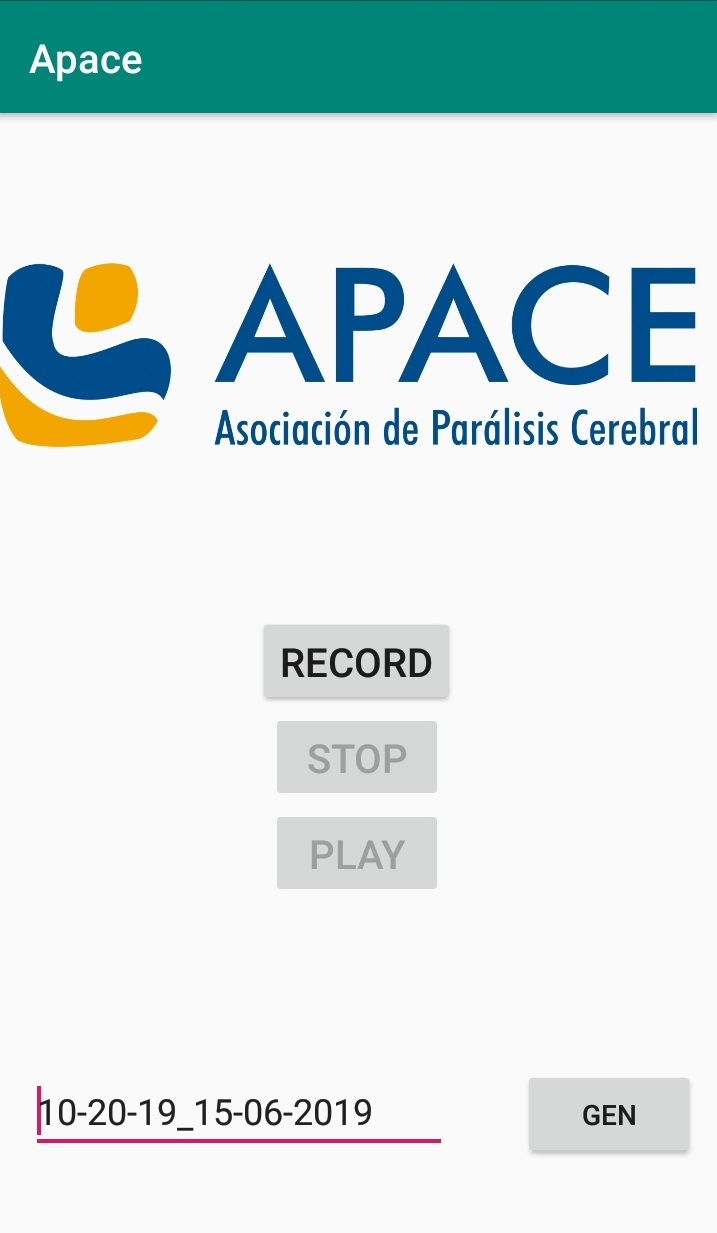
\includegraphics[scale=0.3]{prototipo}
	\caption{Aplicación prototipo.}
	\label{fig:prototipo}
\end{figure}

A la vez que desarrollaba el prototipo estaba investigando acerca de qué formato y qué códec de audio iba mejor para la configuración del \textit{MediaRecorder} y es aquí donde realizamos el estudio del audio. Aquí nos encontramos con el problema de que en \textit{Android} y en concreto con \textit{MediaRecorder} no podíamos codificar, es decir, grabar en cualquier formato. Por ejemplo, vimos que \textit{mp3} con \textit{MediaRecorder} en \textit{Android} solo permite decodificar. Tras realizar el estudio para encontrar el mejor formato, no conseguimos obtener un formato que tuviese un códec sin pérdida, así que intentamos obtener el formato con la mayor calidad posible. Es por ello que elegimos el códec \textit{AAC-LC}, formato \textit{mp4}, con un \textit{bitrate} de 128kbps y un \textit{sampling rate} de 48kHz~\cite{mediarecorder}.

\section{Obtención de las opciones adicionales}
Al comienzo del proyecto se comentó con APACE que quizás los audios no serían suficientes para poder realizar una clasificación exacta de las emociones, pero la clasificación de una respuesta binaria si que se tomaba posible de clasificar solo con el audio. Es por ello que para este problema nos planteamos el uso de unas opciones adicionales que pudiesen dar más información al clasificador.

APACE nos mandó una primera versión de estas opciones adicionales, que se obtuvieron pasando un formulario a las familias de la asociación y a profesionales en la materia. En estas primeras opciones adicionales teníamos un conjunto de opciones por cada una de las emociones que queríamos clasificar, que se pueden ver en la imágenes~\ref{fig:opcdolor}, ~\ref{fig:opcenfado}, ~\ref{fig:opctristeza} y ~\ref{fig:opchambre}. En estas imágenes en la columna de la izquierda están las opciones iniciales, y en la columna derecha las opciones condensadas por APACE. Como se puede observar son demasiadas opciones, tantas que darían demasiadas dimensionalidades a los datos de entrada del clasificador, lo que haría muy complicado el entrenamiento y la clasificación posterior. Es por ello que decidimos tratar de resumir estas opciones, las cuales han sido las que han llegado al final del proyecto y se pueden ver en la tabla~\ref{tabla:opcfinal}.

\begin{figure}
	\centering
	
\includegraphics[width=\textwidth]{dolor}
	\caption{Opciones adicionales proporcionadas por APACE de la emoción dolor.}
	\label{fig:opcdolor}
\end{figure}

\begin{figure}
	\centering
	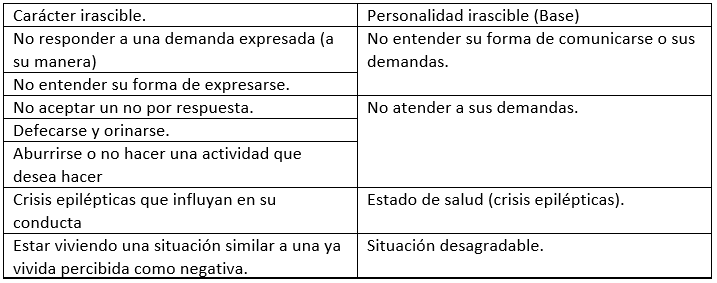
\includegraphics[width=\textwidth]{enfado}
	\caption{Opciones adicionales proporcionadas por APACE de la emoción enfado.}
	\label{fig:opcenfado}
\end{figure}

\begin{figure}
	\centering
	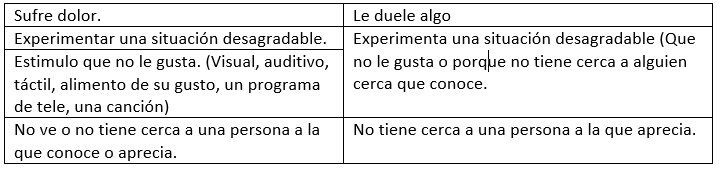
\includegraphics[width=\textwidth]{tristeza}
	\caption{Opciones adicionales proporcionadas por APACE de la emoción tristeza.}
	\label{fig:opctristeza}
\end{figure}

\begin{figure}
	\centering
	
\includegraphics[width=\textwidth]{hambre}
	\caption{Opciones adicionales proporcionadas por APACE de la emoción hambre.}
	\label{fig:opchambre}
\end{figure}

\tablaSmall{Opciones adicionales finales}{l c}{opcfinal}
{ \multicolumn{1}{l}{\textbf{Opción}} & \textbf{Posibles valores} \\}{ 
	Actualmente está enfermo & Sí/No\\
	Sufre dolor crónico & Sí/No\\
	Ha sido operado recientemente & Sí/No\\
	Ha dormido/descansado mal & Sí/No\\
	Ha estado/está en una mala postura & Sí/No\\
	El entorno que lo rodea no es agradable & Sí/No\\
	Las personas que lo rodean no son conocidas & Sí/No\\
	Ha comido & Antes/A su hora/Tarde\\
	Ha comido & Mucho/Normal/Poco/Nada\\
} 

\section{Desarrollo de la aplicación de recogida de datos}
Como ya he comentado, en una reunión con APACE nos transmitieron el cambio que querían hacer en la aplicación prototipo para la recogida de datos, el cual se  que la selección de las opciones adicionales y de la emoción o respuesta relacionada se pudiese hacer desde la aplicación. Con este cambio tuve que empezar a crear la segunda aplicación a partir de la aplicación prototipo. Desde APACE se nos comentó que esta aplicación debía ser lo más sencilla posible de usar, ya que algunas familias, que podían recoger datos, no tienen mucho dominio de las tecnologías. 

Esta aplicación fue bastante más complicada de hacer, ya que era la primera vez que iba a trabajar y tener en cuenta la navegabilidad entre pantallas de la aplicación. Además, la aplicación tenía que ser lo más lineal posible, por lo que primero me puse a diseñar una interfaz, la cual se puede ver en la figura~\ref{fig:interrd}.

Una vez diseñada la interfaz pasé a aprender a navegar por las pantallas de una aplicación \textit{Android} y a desarrollar la aplicación. Del desarrollo de esta aplicación cabe destacar:
\begin{itemize}
	\item Navegabilidad intuitiva gracias al uso de los \textit{ActivityResult}, que permiten terminar un \textit{Activity} con un resultado según ésta haya acabado de forma correcto o incorrecta. Esta funcionalidad la he usado para poder habilitar los botones, ya que se pidió que la aplicación fuese simple y lineal.
	\item En la pantalla de selección de la emoción o respuesta relacionada con los datos generados no se permite ni dejarla vacía, ni elegir una opción de la columna de emociones y otra de la columna respuesta, ni elegir las opciones sí y no de forma simultanea.
	\item Uso de ficheros \textit{csv} para la almacenar y enviar tanto las opciones adicionales como la emoción o respuesta asociado, usando la librería \textit{OpenCSV}~\cite{opencsv}.
	\item Persistencia y carga de los datos en todas las pantallas gracias a una creación de carpetas bien definidas y al uso de una estructura de datos bien definida. Esto nos permite volver a entrar a una de las pantallas y tener los datos que se habían generado. Ocurre tanto en la pantalla de grabación del audio, como en las pantallas de selección de opciones y de selección de emoción o respuesta.
	\item Generación de comprimidos con el archivo del audio y los archivos \textit{csv}, para poder enviarlos con mayor facilidad.
	\item Envío por correo del comprimido para poder recogerlo y estudiarlo. 
\end{itemize}

Este último punto hubo que discutirlo con los tutores, porque nuestras opciones para enviar el comprimido eran o hacerlo directamente con un servidor o usar un correo electrónico. Al final, decidimos usar el correo electrónico ya que no teníamos tiempo de desplegar un servidor y la aplicación tenía que estar en marcha lo antes posible para que se empezase a generar datos con los que el investigador colaborador, Sergio Chico, pudiese hacer el estudio.

Además, un problema habitual en el desarrollo de servidores en los trabajos fin de grado es que al finalizar estos los datos almacenados en ellos se pierden. Esto puede ser muy importante, ya que en años posteriores otro alumno puedo partir de ese Trabajo Fin de Grado, pero ya no tendría datos. Esta es una ventaja más del uso del correo, ya que por mucho que se desconecte el servidor, siempre se puede acceder a los datos almacenados en el correo, por lo que nunca se pierden.

La interfaz final de la aplicación se puede ver en la figura~\ref{fig:interfinalrd}.
\begin{figure}
	\centering
	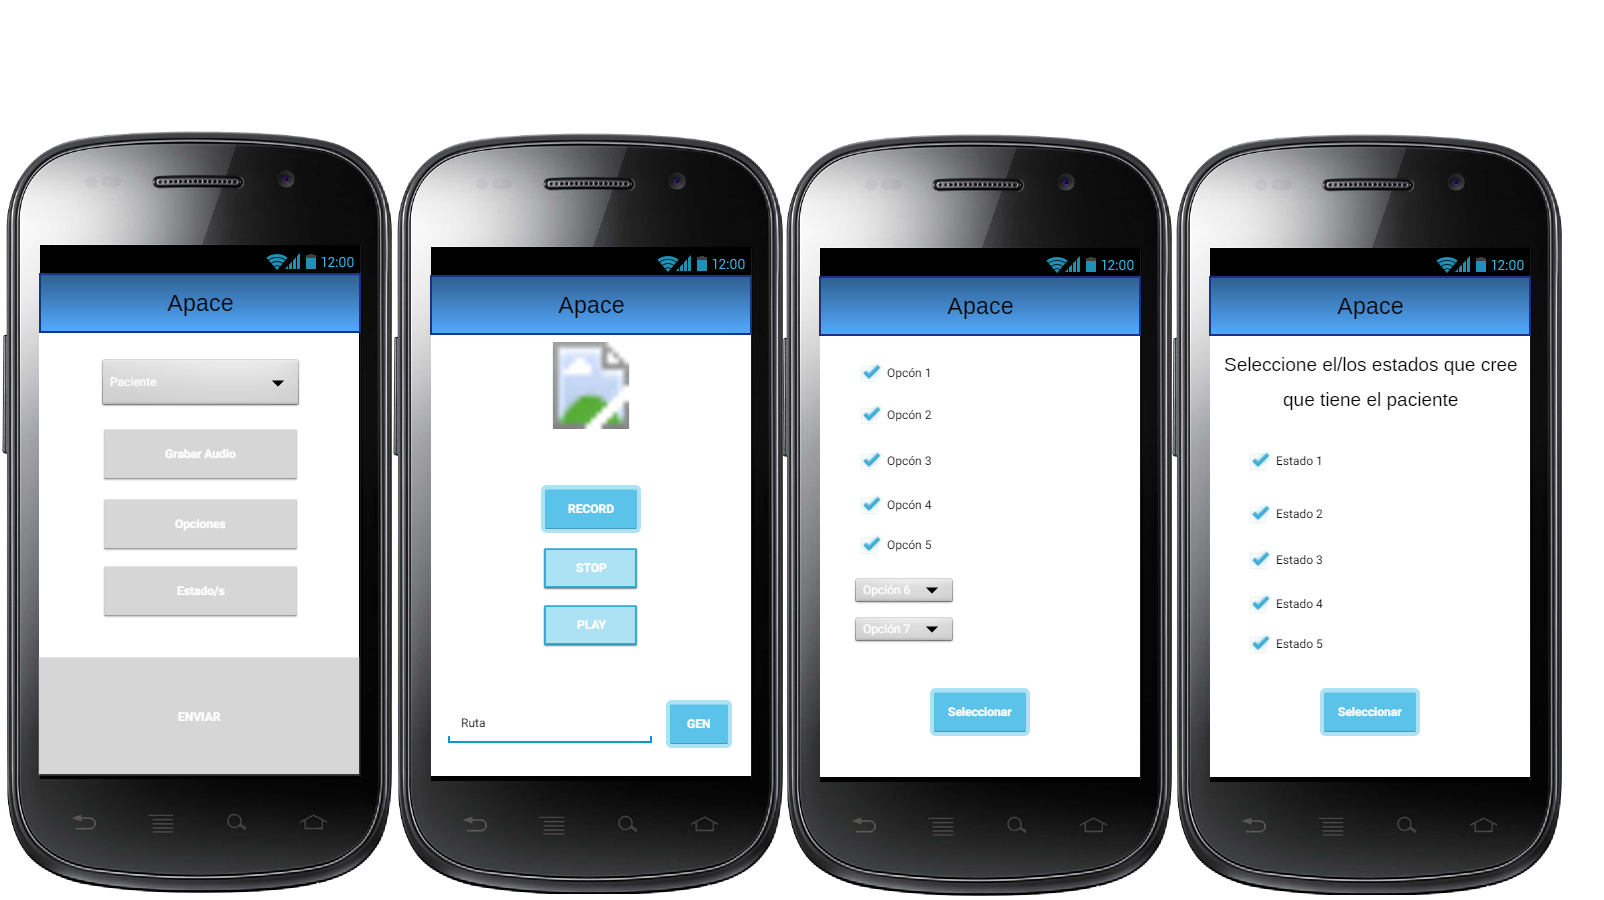
\includegraphics[width=\textwidth]{interfaz}
	\caption{Diseño interfaz aplicación recogida de datos.}
	\label{fig:interrd}
\end{figure}
\begin{figure}
	\centering
	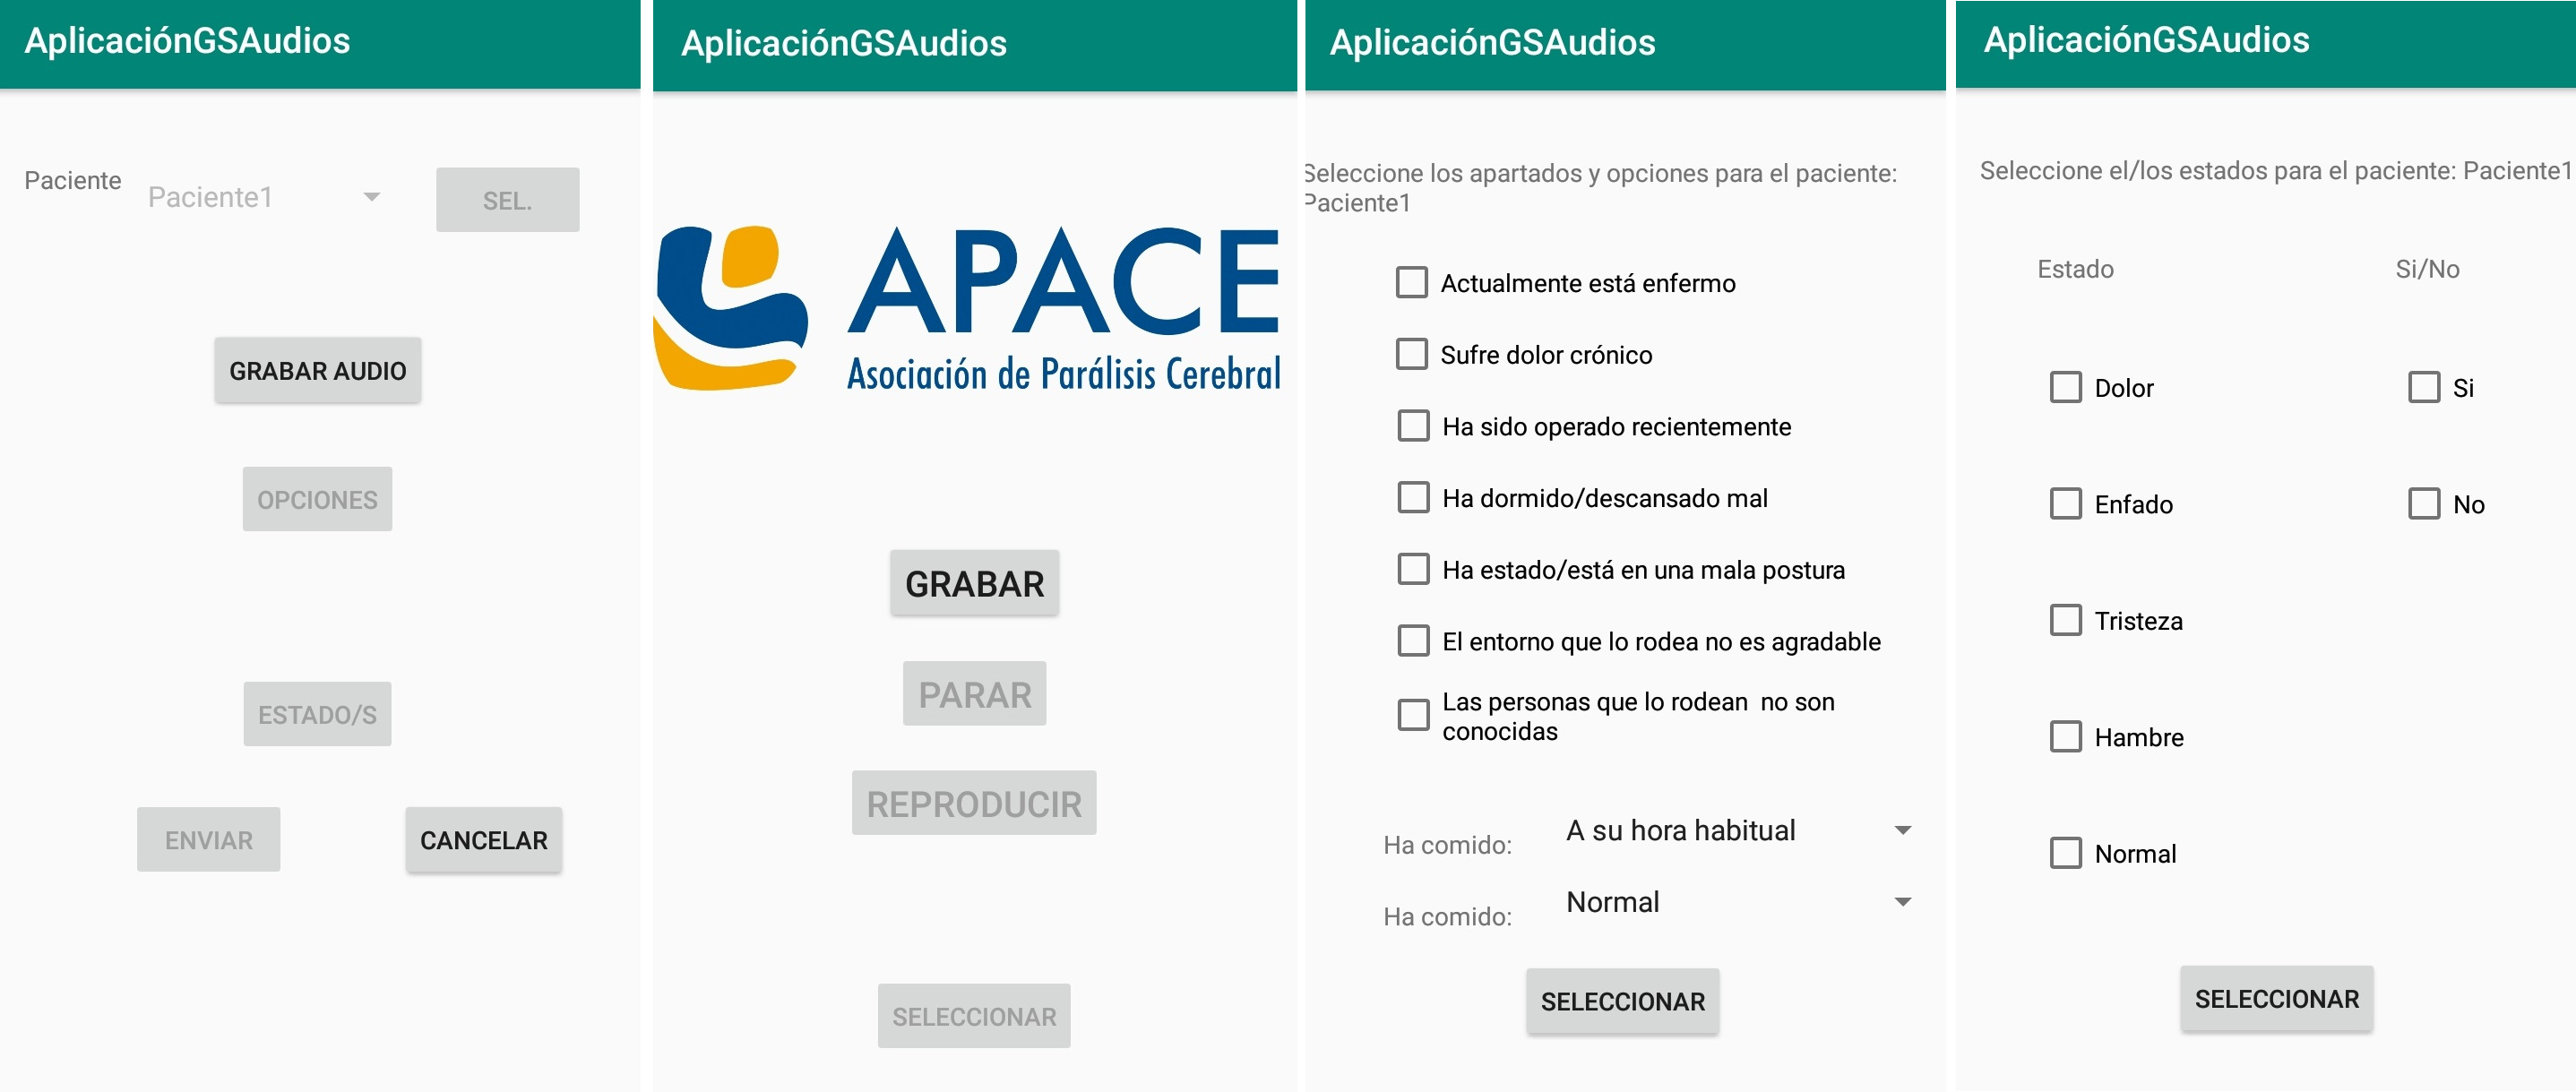
\includegraphics[width=\textwidth]{interfinalrd}
	\caption{Interfaz aplicación recogida de datos.}
	\label{fig:interfinalrd}
\end{figure}

\section{Obtención de sonidos prototipo}
Tras finalizar la aplicación para la generación de datos, y sus presentaciones en APACE que posteriormente comentaré, nos encontramos con un problema que ya veíamos venir desde prácticamente el comienzo del proyecto, la falta de datos. Obviamente no podíamos forzar a los pacientes a hacer sonidos, y menos cuando las emociones con las que nos pidió APACE trabajar son negativas (dolor, hambre, tristeza y enfado).

En una reunión comentamos las posibles opciones que teníamos, y éstas eran o esperar a que antes de la entrega tuviésemos suficientes datos como para al menos tener un clasificador para una persona, o intentar imitar los sonidos para poder generar algunos datos con los que el investigador colaborador, Sergio Chico, pudiese empezar a trabajar. Con el fin de poder tener una aplicación prototipo final que nos permitiese clasificar audios decidí generar de forma artificial los audios con los que entrenar al clasificador.

Esta probablemente sea una de las tareas que más me ha costado en todo el proyecto, ya que tenía que seguir unos pasos, para que los datos que generase tuviesen el mayor sentido posible. Estos pasos para cada una de las emociones y sí/no eran:
\begin{itemize}
	\item Descargar algunos ejemplos que ya hubiesen enviado, para tener algo en lo que basarme.
	\item Grabar un audio propio intentando ceñirme lo máximo posible a los audios descargados anteriormente.
	\item En las emociones, estudiar las opciones adicionales para saber cuales se suelen repetir más con una emoción.
	\item Grabar alrededor de unos 20 audios por cada emoción y sí/no, teniendo que escucharlos, valorar si son o no válidos y poner las opciones adicionales correspondientes para cada una de la grabaciones.
\end{itemize}
\section{Desarrollo de la aplicación de interpretación - AVC}
Una vez que ya contábamos con suficientes datos como para que el investigador colaborador, Sergio Chico, empezase a estudiar las mejores formas de extraer las características del audio y poder clasificarlo, yo empecé a desarrollar la aplicación final. Es la aplicación más importante en el proyecto, ya que es la que se más se usará y la que dará esa mejora en la vida de las personas con parálisis cerebral que buscamos.

Lo primero que realicé fue el diseño de la interfaz junto con un equipo especializado de APACE. Diseñé al rededor de 6 interfaces iniciales, en las cuales se destaca el uso desde el principio de botones de información para dar mayor accesibilidad a la aplicación, y para las cuales este equipo me fue indicando cambios y mejoras hasta llegar al diseño final, que aparece en la figura~\ref{fig:dinteravc}. 

Cabe destacar un cambio muy importante que me comentaron desde APACE, y es que las opciones adicionales no se cumplimentasen cada vez que queremos hacer una interpretación, sino que estas se almacenasen en el servidor y solo se modificasen cuando sea necesario.

\begin{figure}
	\centering
	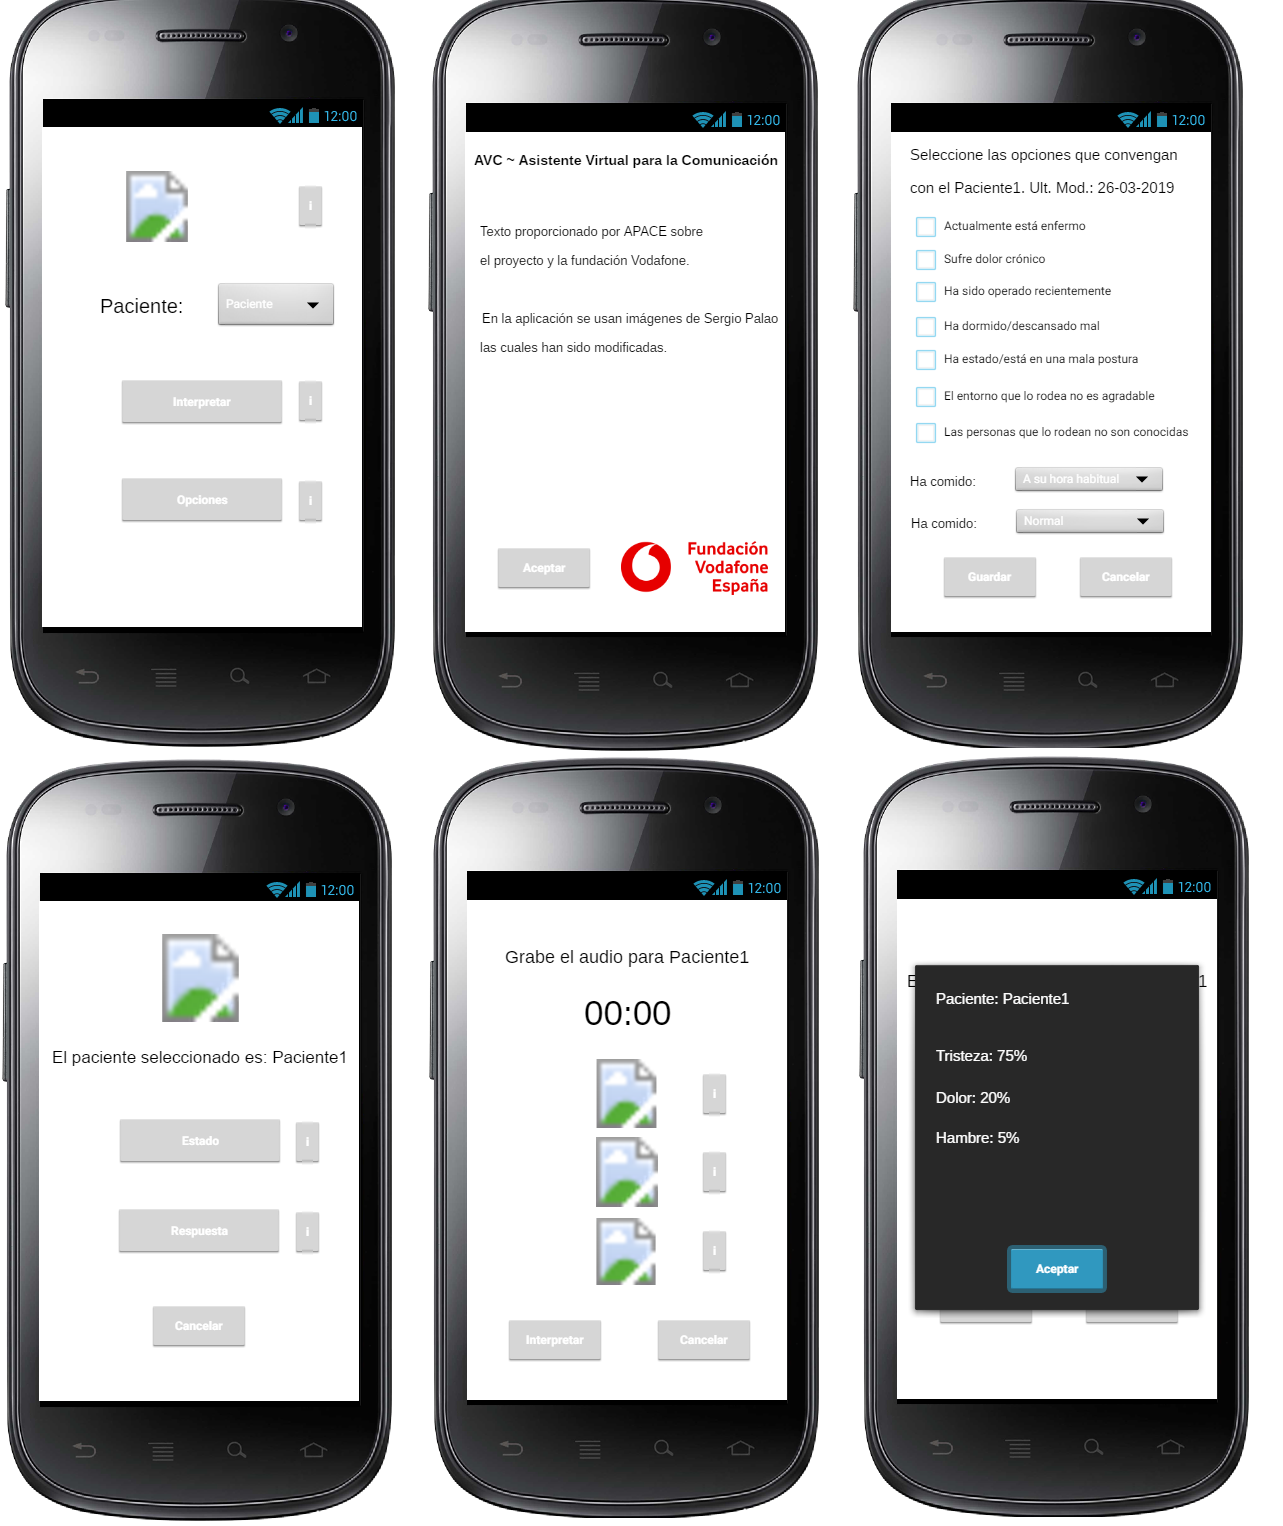
\includegraphics[width=\textwidth]{disintavc}
	\caption{Diseño interfaz aplicación AVC.}
	\label{fig:dinteravc}
\end{figure}

Esta es la aplicación más importante y compleja del proyecto. Es por ello que es a la que sin duda he dedicado más tiempo. En el desarrollo de esta primera versión sin conexión al servidor cabe destacar los siguientes apartados:
\begin{itemize}
	\item \textbf{Creación de una estructura de ficheros:} necesario para poder controlar los distintos ficheros con los que trabaja la aplicación, siendo la raíz de esta estructura donde se almacena el audio grabado. En la carpeta \textit{/config} tenemos el fichero \textit{csv} donde se almacena al paciente por defecto.
	\item \textbf{Comprobación y restauración de la estructura de ficheros}: para que al iniciarse la aplicación lo primero que se compruebe sea que la estructura de ficheros existe, y si falta alguna carpeta y/o fichero los genere.
	\item \textbf{Implementación de la selección del paciente por defecto:} que al abrir de nuevo la aplicación aparezca en el \textit{spinner} del paciente el último paciente seleccionado antes de cerrar la aplicación. Esto se ha conseguido gracias al conocimiento sobre el control de ficheros \textit{csv} obtenido en el desarrollo de la aplicación de generación de datos con \textit{OpenCSV}~\cite{opencsv}.
	\item \textbf{Continua implicación por parte de APACE:} necesaria para conseguir que la aplicación fuese lo más accesible posible. Esto dio como resultado algunos cambios en la interfaz, desde las primeras versiones que aparecen en la figura~\ref{fig:primver} donde me comentaron que los degradados no eran lo mejor para personas con alguna discapacidad visual, a una segunda versión donde, a parte de eliminar el degradado, se modificó el color al color que ellos me dijeron, que era el azul, teniendo así que modificar todas las imágenes para que los textos estuviesen en blanco~\ref{fig:segver}. Por último, eliminé todos los píxeles blancos de las imágenes a mano, porque al tener las imágenes con un fondo azul los píxeles blancos se ven mucho. Esto nos lleva a la última versión de la interfaz~\ref{fig:verfi}.
	\item \textbf{Uso de diálogos para mejorar la accesibilidad:} con \textit{AlerDialog} en los botones de información para mostrar información sobre el botón que está al lado. Estos diálogos están escritos en lectura fácil gracias a la Universidad de Salamanca. Además, al abrir el diálogo se reproduce por audio el texto escrito para dar una mayor accesibilidad~\ref{fig:dia}.
\end{itemize}
Como se puede observar, el desarrollo de esta aplicación ha sido orientado casi totalmente a conseguir una mayor accesibilidad. Este punto ha sido tan importante en el equipo de desarrollo porque desde un principio teníamos la idea de que hasta los compañeros de estas personas gravemente afectadas del centro de día de APACE pudiesen utilizarlo, para así poder entender a sus compañeros.

\begin{figure}
	\centering
	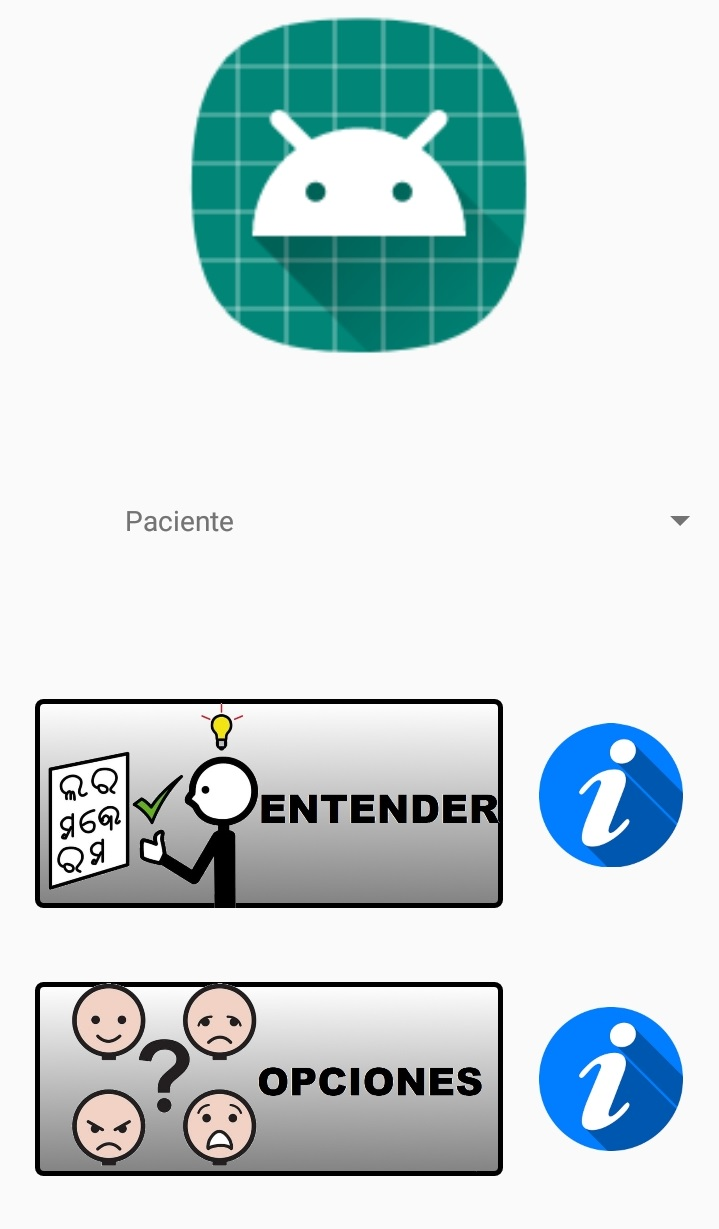
\includegraphics[scale=0.3]{primerasversiones}
	\caption{Primera versión de la interfaz.}
	\label{fig:primver}
\end{figure}
\begin{figure}
	\centering
	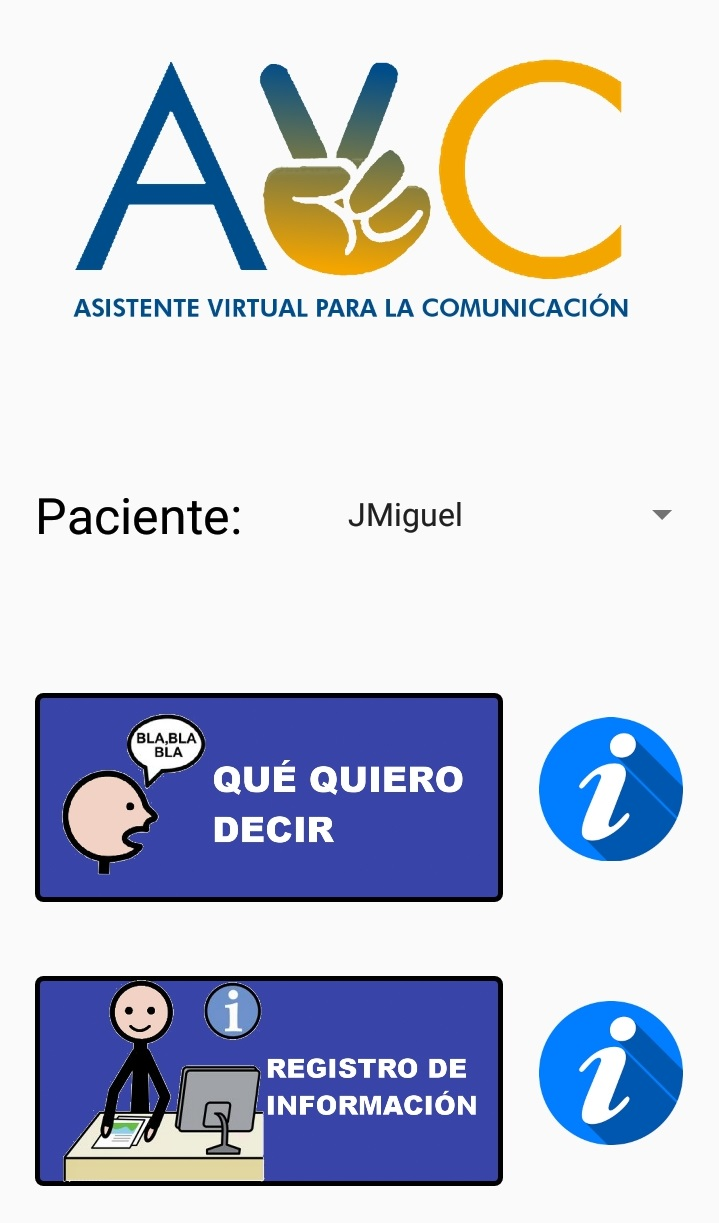
\includegraphics[scale=0.3]{segundaversion}
	\caption{Segunda versión de la interfaz.}
	\label{fig:segver}
\end{figure}
\begin{figure}
	\centering
	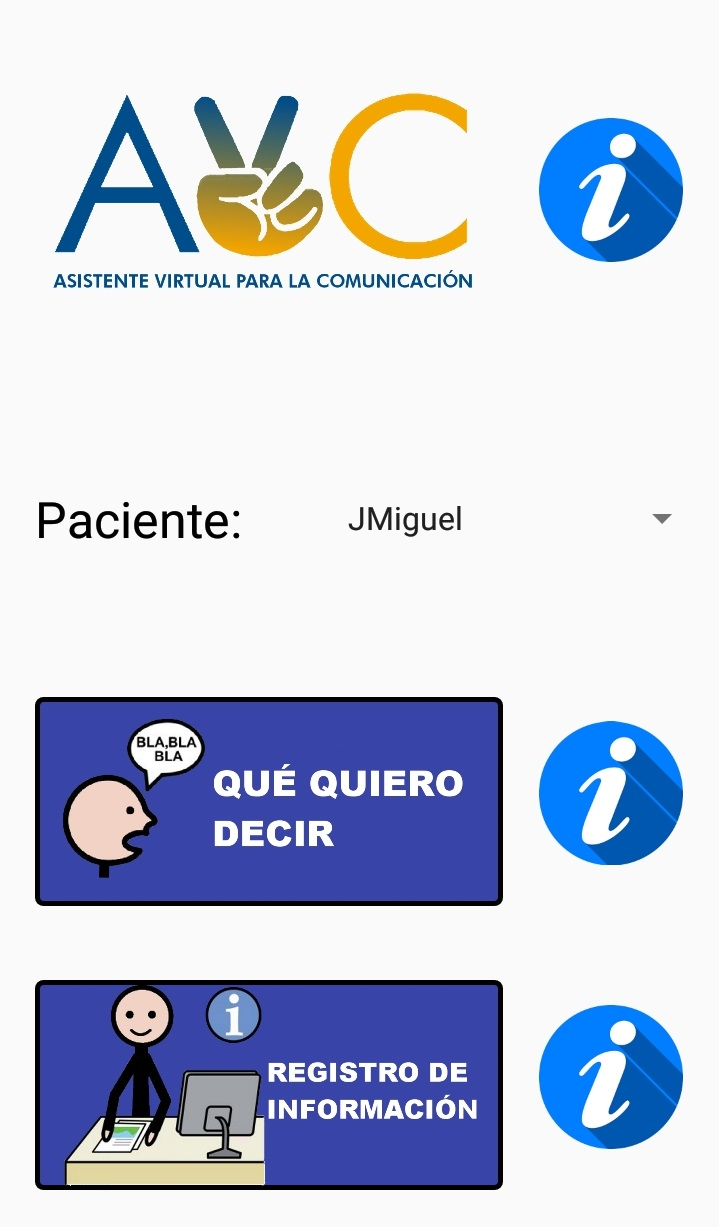
\includegraphics[scale=0.3]{versionfinal}
	\caption{Versión final de la interfaz, donde no se observan los bordes blancos en los pictogramas, como se puede ver en la segunda versión.}
	\label{fig:verfi}
\end{figure}
\begin{figure}
	\centering
	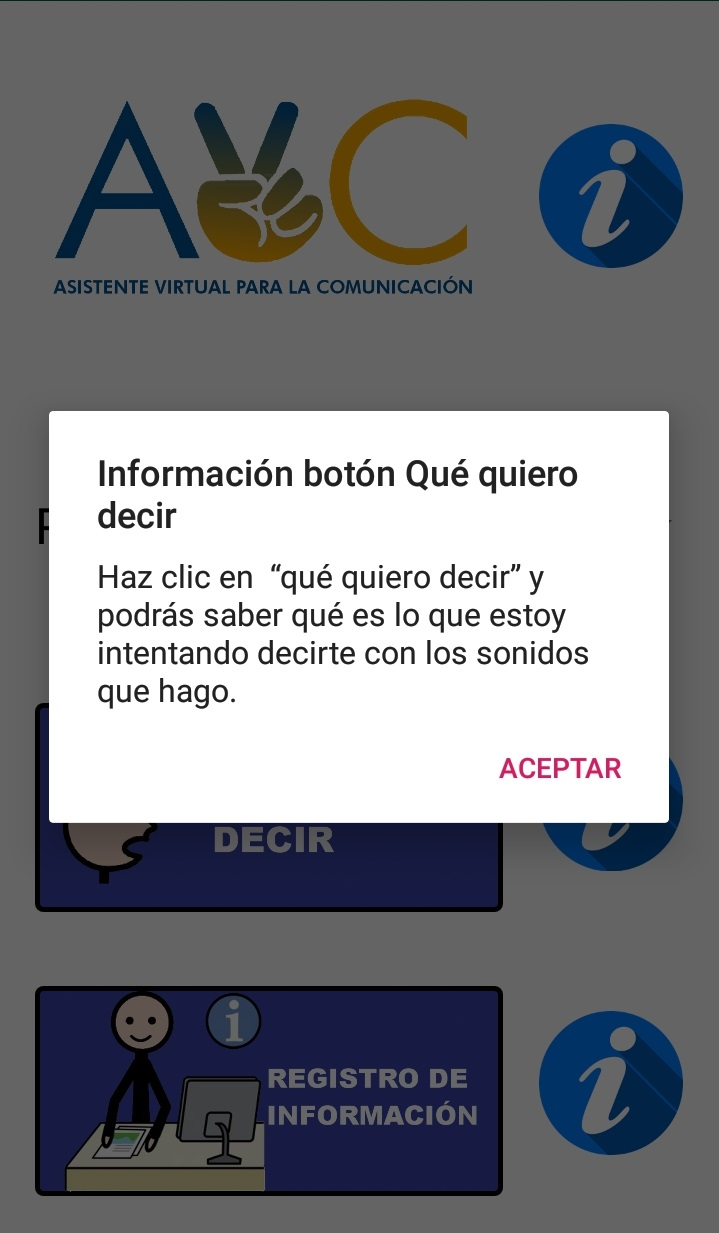
\includegraphics[scale=0.3]{dialogo}
	\caption{Ejemplo de diálogo en lectura fácil.}
	\label{fig:dia}
\end{figure}

Después de terminar el desarrollo de la aplicación empecé con la fase de test de ésta. En ella primero diseñé los test unitarios para probar la lógica y la creación de los distintos elementos de la aplicación y los implementé, y después, usando Espresso~\cite{espresso}, diseñé e implementé los test de integración para comprobar la correcta colaboración entre las distintas partes de la aplicación. Un ejemplo de este diseño de los test se puede ver en la figura~\ref{fig:ditestun}~\cite{vypcn,vypcb,vypti}.

\begin{figure}
	\centering
	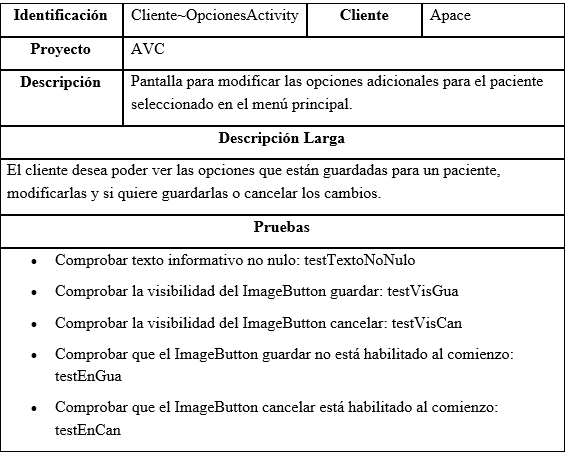
\includegraphics[width=\textwidth]{distest}
	\caption{Diseño de test unitarios de OpcionesActivity.}
	\label{fig:ditestun}
\end{figure}

Tras probar los distintos test descubrí unos cuantos \textit{bugs}, que es la función de los test. Hubo un \textit{bug} en particular que me llevó mucho tiempo resolver, el cual afectaba a cómo se generaba la estructura de datos, ya que hay algunos test que prueban esa funcionalidad eliminando partes o toda la estructura de ficheros de la aplicación.

Además, realicé un tipo especial de test llamado \textit{Monkey Test}~\cite{monkeytest}, que consiste en, a través de una prueba de estrés pulsando aleatoriamente puntos de la pantalla, probar la consistencia de la aplicación. Gracias a este test descubrí un error importante en la pantalla de grabación de audios, ya que la grabación no se paraba cuando se retrocedía a la pantalla anterior pulsando el botón \textit{back} del dispositivo.
\section{Desarrollo del servidor}
Tras tener una primera versión de la aplicación tocaba empezar a desarrollar el servidor. Para ello primero tenía que aprender a usar \textit{Flask}~\cite{flask}, ya que era la primera vez que iba a desarrollar un servidor.

El primer paso que tuve que dar fue el de elegir el tipo de \textit{request} con el cual quería hacer las peticiones al servidor. Elegí el tipo \textit{post} porque tenía más conocimiento acerca de este tipo de \textit{request HTTP} y por recomendación de compañeros~\cite{sdintro,sdhttp}.

El segundo paso fue el diseño de los distintos métodos del servidor. Tras el diseño se decidí usar 4 métodos \textit{post} en el servidor:
\begin{itemize}
	\item \textbf{Nombre:} API/Nombres, \textbf{caso de uso:} CU1, \textbf{descripción:} Devuelve la lista de usuarios de los que hay un método entrenado preparado para clasificar. Esta lista está en un fichero csv en el servidor, \textbf{parámetros:} Token, \textbf{salida:} JSON con una cadena con la lista de los nombres.
	\item \textbf{Nombre:} API/ObtOpciones, \textbf{caso de uso:} CU2, \textbf{descripción:} Devuelve los valores de las opciones adicionales del paciente seleccionado, leyendo el fichero csv del servidor indicado, \textbf{parámetros:} Paciente y token, \textbf{salida:} JSON con una cadena con la lista de las opciones almacenadas.
	\item \textbf{Nombre:} API/GuaOpciones, \textbf{caso de uso:} CU3, \textbf{descripción:} Almacena las opciones que se envían desde la aplicación para el paciente seleccionado, \textbf{parámetros:} Paciente, lista de valores y token, \textbf{salida:} Resultado booleano de la operación.
	\item \textbf{Nombre:} API/Clasifica, \textbf{caso de uso:} CU5 y CU6, \textbf{descripción:} Ejecuta el modelo entrenado para el paciente pasado con el audio pasado y con las opciones adicionales que están actualmente guardadas en el servidor., \textbf{parámetros:} Paciente, tipo de interpretación, audio y token, \textbf{salida:} JSON con una cadena con los datos sobre la emoción o respuesta y sus porcentajes.
\end{itemize}

Después, cree la estructura necesaria en el servidor, esta estructura es:

\dirtree{%
	.1 root.
	.2 Modelos.
	.2 Opciones.
	.2 Temp.
	.2 pacientes.csv.
	.2 apiserver.py.
	.2 clip.py.
}

En la carpeta \textit{Modelos} es donde se almacenan los distintos modelos ya entrenados. En la carpeta \textit{Opciones} se encuentran todos los \textit{csv} con las opciones adicionales guardadas para cada paciente. En \textit{Temp} tenemos los ficheros de audio temporales de cada interpretación, éstos se eliminarán después de devolver al cliente el resultado. El fichero \textit{pacientes.csv} tiene la lista de pacientes entrenados y los ficheros \textit{apiserver.py} y \textit{clip.py} son los ficheros encargados de la extracción de características y de la clasificación.

Por último, implementé todos los métodos en \textit{Python}, haciendo todas las respuestas con \textit{jsonify}~\cite{jsonify}. Algunos aspectos que se pueden destacar del desarrollo del servidor son:
\begin{itemize}
	\item \textbf{Control de concurrencia:} sobre todo en el método de clasificación donde el servidor recibe varios archivos de audios que tiene que saber identificar correctamente. Esto se ha conseguido gracias a la creación dinámica de nombres para los audios en el servidor.
	\item \textbf{Resultado aleatorio:} a parte de obviamente tener el clasificador para los datos que generé, quise añadir más usuarios en la aplicación para así poder modificar las opciones y comprobar el correcto funcionamiento, pero para ello también necesitaba un clasificador para estos audios. Es por ello que creé una función que genera resultados válidos aleatorios con los cuales responder a las interpretaciones de pacientes no entrenados.
\end{itemize}

Tras haber implementado cada uno de los métodos tenía que probarlo, pero como la aplicación final no estaba desarrollada, puesto que aun no estaban unidas ambas partes, aplicación y servidor, tuve que usar una herramienta para poder hacer \textit{request HTTP} desde el ordenador.

\section{Conexión de aplicación y servidor}
Una vez tuve la aplicación y el servidor desarrollados solo quedaba unir ambas partes. Para ello primero tuve que aprender a realizar \textit{post} en \textit{Android}. Decidí hacer los \textit{post} con paso de parámetros por \textit{url}, lo que después me llevó un problema con el audio que contaré posteriormente.

Al implementar los métodos \textit{post} me encontré con un problema. La conexión al servidor, que está desplegado en un portátil al cual tengo que acceder a través de una dirección IP. Eso cuando lo estaba implementando en casa era sencillo, ya que esta IP apenas cambiaba y solo hay un router en red, pero la presentación del proyecto se iba a hacer en sitios como la universidad, o el mismo APACE, donde nos encontramos con redes más complejas donde apuntar a un dispositivo no es tan fácil como poner la IP. Es por ello que decidí usar el programa \textit{noWifi} en el portátil en donde está desplegado el servidor, ya que me permite crear un red a la cual apuntar con los dispositivos \textit{Android} siempre con la dirección 192.168.137.1 y al puerto definido en \textit{Flask}, el puerto 5000.

Al implementar el cuarto método \textit{post} en \textit{Android}, el método que me permite enviar la petición de clasificación, me encontré con un gran problema. ¿Cómo conseguir pasar un archivo de audio en \textit{mp4} a un servidor a través de un método en el cual le paso los parámetros por texto en la \textit{url}? La respuesta la encontré en la codificación a \textit{Base64}, que me permite transformar mi archivo de audio en texto, el cual puedo pasar en la \textit{url} y luego decodificarlo en el servidor haciendo la operación inversa. 

Al desarrollar el paso a \textit{Base64} me encontré con otro problema, puesto que la codificación que usaba en \textit{Android} no se decodificaba bien en el servidor \textit{Python}. Me llevó mucho tiempo solventarlo, ya que intenté usar muchos métodos para codificar en \textit{Base64}, pero ninguno daba resultado porque todos los métodos que probaba al decodificarlo en el servidor me daba como resultado un fichero corrupto. Además, se juntó otro impedimento, y es que la librería de \textit{Base64} de \textit{Java} subía el API mínimo varias versiones, por lo que de usarlo no podríamos cumplir nuestro objetivo técnico de usar como máximo la API 23 de \textit{Android}~\cite{base64java}. Tras probar muchos métodos pasé directamente a imprimir el resultado de la codificación para ver si podía verse el problema, y en efecto, no se correspondía con la codificación esperada por el servidor. Fue entonces cuando cambié el fichero de audio para pasar a codificar un fichero de texto, encontré el método, \textit{Base64.encodeToString} que funcionaba correctamente en \textit{Android}, y luego lo probé con el fichero de audio y por fin funcionó.

\begin{lstlisting}[language={Java}]
String baudio=null;

try {
	byte[] b = new byte[(int) aufile.length()];
	FileInputStream fis = new FileInputStream(aufile);
	fis.read(b);
	baudio = Base64.encodeToString(b, Base64.NO_WRAP);
} catch (FileNotFoundException e) {
	e.printStackTrace();
} catch (IOException e) {
	e.printStackTrace();
}	
\end{lstlisting}

En el código se ve como se hace la codificación a \textit{Base64}. Es importante el uso del \textit{Base64.NO\_WRAP}, ya que lo que hace es codificarlo todo como una única cadena, debido a que otras configuraciones lo que hacen es introducir saltos de línea que impiden la correcta decodificación.

Por último, quise dar una mayor seguridad al servidor para que no se pueda acceder a una de las peticiones desde fuera de la aplicación. Esto lo conseguí añadiendo un \textit{token} de seguridad como parámetro a todos los métodos. Fue entonces cuando pensé que puede haber una serie de errores con el servidor que se podrían agrupar, codificar, describir y dar una solución. Es así como se me ocurrió hacer una estandarización de los errores de la aplicación en la conexión con el servidor. Estos tienen un código asociado, y con él una descripción de por qué ocurre y como solucionarlo, como se ve en la tabla~\ref{tabla:errores}. Un ejemplo de un mensaje de error se puede ver en la figura~\ref{fig:error}.
	
\begin{table}
	\resizebox{\textwidth}{!}{%
		\begin{tabular}{@{}llll@{}}
			\toprule
			Error & \textbf{Descripción}                                                                & \textbf{Causa}                                                                                                                                                                               & \textbf{Solución}                                                                                                                                    \\ \midrule
			Er1   & \begin{tabular}[c]{@{}l@{}}No se puede \\ acceder al servidor.\end{tabular}         & \begin{tabular}[c]{@{}l@{}}Este error se da cuando el servidor\\  está caído.\end{tabular}                                                                                                   & \begin{tabular}[c]{@{}l@{}}Avisar al Administrador para que \\ reinicie el servidor.\end{tabular}                                                    \\
			Er2   & \begin{tabular}[c]{@{}l@{}}Token de \\ seguridad\\  incorrecto.\end{tabular}        & \begin{tabular}[c]{@{}l@{}}O se ha corrompido la aplicación\\  cambiando el token de seguridad \\ o el token de seguridad ha cambiado\\  sin ser actualizado en su dispositivo.\end{tabular} & \begin{tabular}[c]{@{}l@{}}Avisar al Administrador para que \\ le pase de nuevo la aplicación.\end{tabular}                                          \\
			Er3   & \begin{tabular}[c]{@{}l@{}}Lista de nombres \\ vacía en el servidor.\end{tabular}   & \begin{tabular}[c]{@{}l@{}}La lista con los nombres en el\\  servidor está vacía.\end{tabular}                                                                                               & \begin{tabular}[c]{@{}l@{}}Avisar al Administrador para \\ que recupere el archivo.\end{tabular}                                                     \\
			Er4   & \begin{tabular}[c]{@{}l@{}}Lista de nombres \\ no encontrada.\end{tabular}          & \begin{tabular}[c]{@{}l@{}}El fichero con la lista de los \\ pacientes en el servidor no está.\end{tabular}                                                                                  & \begin{tabular}[c]{@{}l@{}}Avisar al Administrador para \\ que recupere el archivo.\end{tabular}                                                     \\
			Er5   & \begin{tabular}[c]{@{}l@{}}Opciones del \\ paciente no\\  encontradas.\end{tabular} & \begin{tabular}[c]{@{}l@{}}El fichero con las opciones \\ adicionales del paciente no \\ está en el servidor.\end{tabular}                                                                   & \begin{tabular}[c]{@{}l@{}}Avisar al Administrador para \\ que recupere el archivo.\end{tabular}                                                     \\
			Er6   & \begin{tabular}[c]{@{}l@{}}No hay \\ conexión \\ a Internet.\end{tabular}           & \begin{tabular}[c]{@{}l@{}}No tener conexión ni Wifi \\ ni Datos Móviles.\end{tabular}                                                                                                       & \begin{tabular}[c]{@{}l@{}}Conectarse a una red con acceso\\  a Internet.\end{tabular}                                                               \\
			Er7   & \begin{tabular}[c]{@{}l@{}}Fichero del \\ paciente vacío.\end{tabular}              & \begin{tabular}[c]{@{}l@{}}El fichero del paciente con las\\  opciones está vacío en el servidor.\end{tabular}                                                                               & \begin{tabular}[c]{@{}l@{}}Avisar al Administrador para \\ que recupere el archivo.\end{tabular}                                                     \\
			Er8   & \begin{tabular}[c]{@{}l@{}}Fichero de \\ clasificación \\ no existe.\end{tabular}   & \begin{tabular}[c]{@{}l@{}}No existe el fichero con el que se\\  clasifica en el servidor a ese paciente.\end{tabular}                                                                       & \begin{tabular}[c]{@{}l@{}}Avisar al Administrador para \\ que recupere el archivo.\end{tabular}                                                     \\
			Er9   & Resultado vacío.                                                                    & \begin{tabular}[c]{@{}l@{}}El servidor ha devuelto una \\ solución vacía.\end{tabular}                                                                                                       & \begin{tabular}[c]{@{}l@{}}Avisar al Administrador para \\ que compruebe el funcionamiento \\ de la clasificación para ese\\  paciente.\end{tabular} \\ \bottomrule
		\end{tabular}
	}
	\caption{Código de errores.}
	\label{tabla:errores}
\end{table}

\begin{figure}
	\centering
	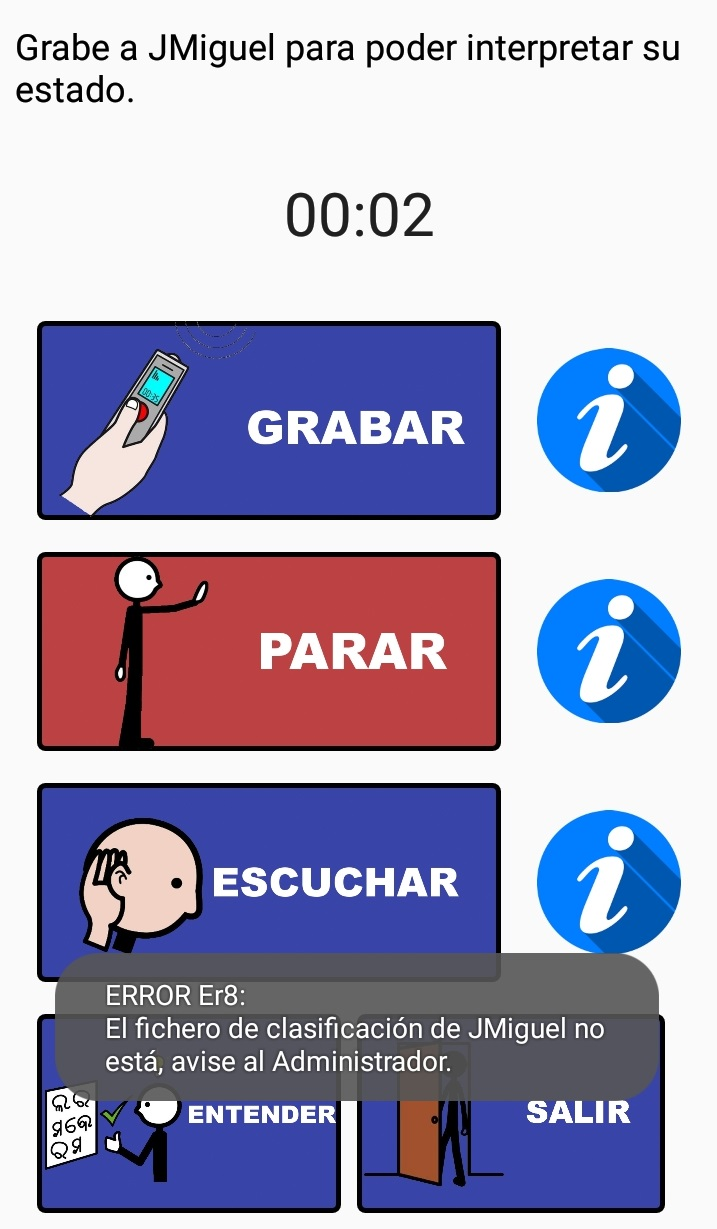
\includegraphics[scale=0.3]{error}
	\caption{Ejemplo de error.}
	\label{fig:error}
\end{figure}

Después de terminar de enlazar la aplicación de interpretación con el servidor, modifiqué y eliminé algunos test que tenía implementados, pudiendo así probar desde los test unitario y de integración el servidor. Al final, realicé un total de 82 test, como se puede ver en la figura~\ref{fig:test}, entre unitario y de integración, que prueban diferentes partes de la aplicación y el servidor.

\begin{figure}
	\centering
	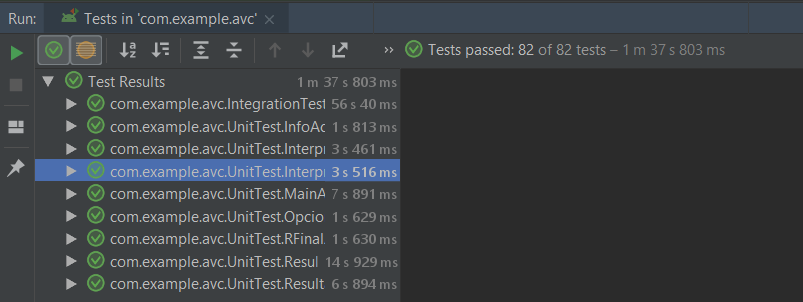
\includegraphics[width=\textwidth]{test}
	\caption{Resultado de los 82 test.}
	\label{fig:test}
\end{figure}

Con esto terminé el desarrollo de código del proyecto, pero no el proyecto en general ya que aún quedaba realizar presentaciones y documentarlo.

\section{Presentaciones y Premios}
Desde un principio nos pusimos como objetivo en el proyecto que éste fuese mediático, es decir, intentar apuntarnos al mayor número de presentaciones donde poder mostrar los avances del proyecto. A lo largo del desarrollo del proyecto he realizado, a diferentes tipos de públicos, las siguientes presentaciones:
\begin{itemize}
	\item Varias presentaciones en APACE de la aplicación de recogida de datos a los familiares y cuidadores del centro.
	\item Presentación de la aplicación final en las jornadas ASPACEnet en Madrid, 28 de Mayo de 2019. El certificado de asistencia se puede ver en la figura~\ref{fig:madrid}.
	\item Presentación para la elaboración del vídeo final del proyecto, \url{https://www.youtube.com/watch?v=6lWLMS9o8v0&feature=youtu.be}.
	\item Presentación de la aplicación final a los cuidadores del centro.
	\item Presentación ante la prensa del proyecto y de la aplicación~\ref{fig:presprensa}, la nota de prensa presencial se puede ver después de las líneas de trabajo futuras en el último apartado, y la nota de prensa digital se puede ver en  \url{https://www.diariodeburgos.es/Noticia/Z2D22B97F-0523-981F-1046FF5A06C5B81F/201906/Una-aplicacion-para-entender-a-quienes-no-pueden-hablar}.
\end{itemize}

\begin{figure}
	\centering
	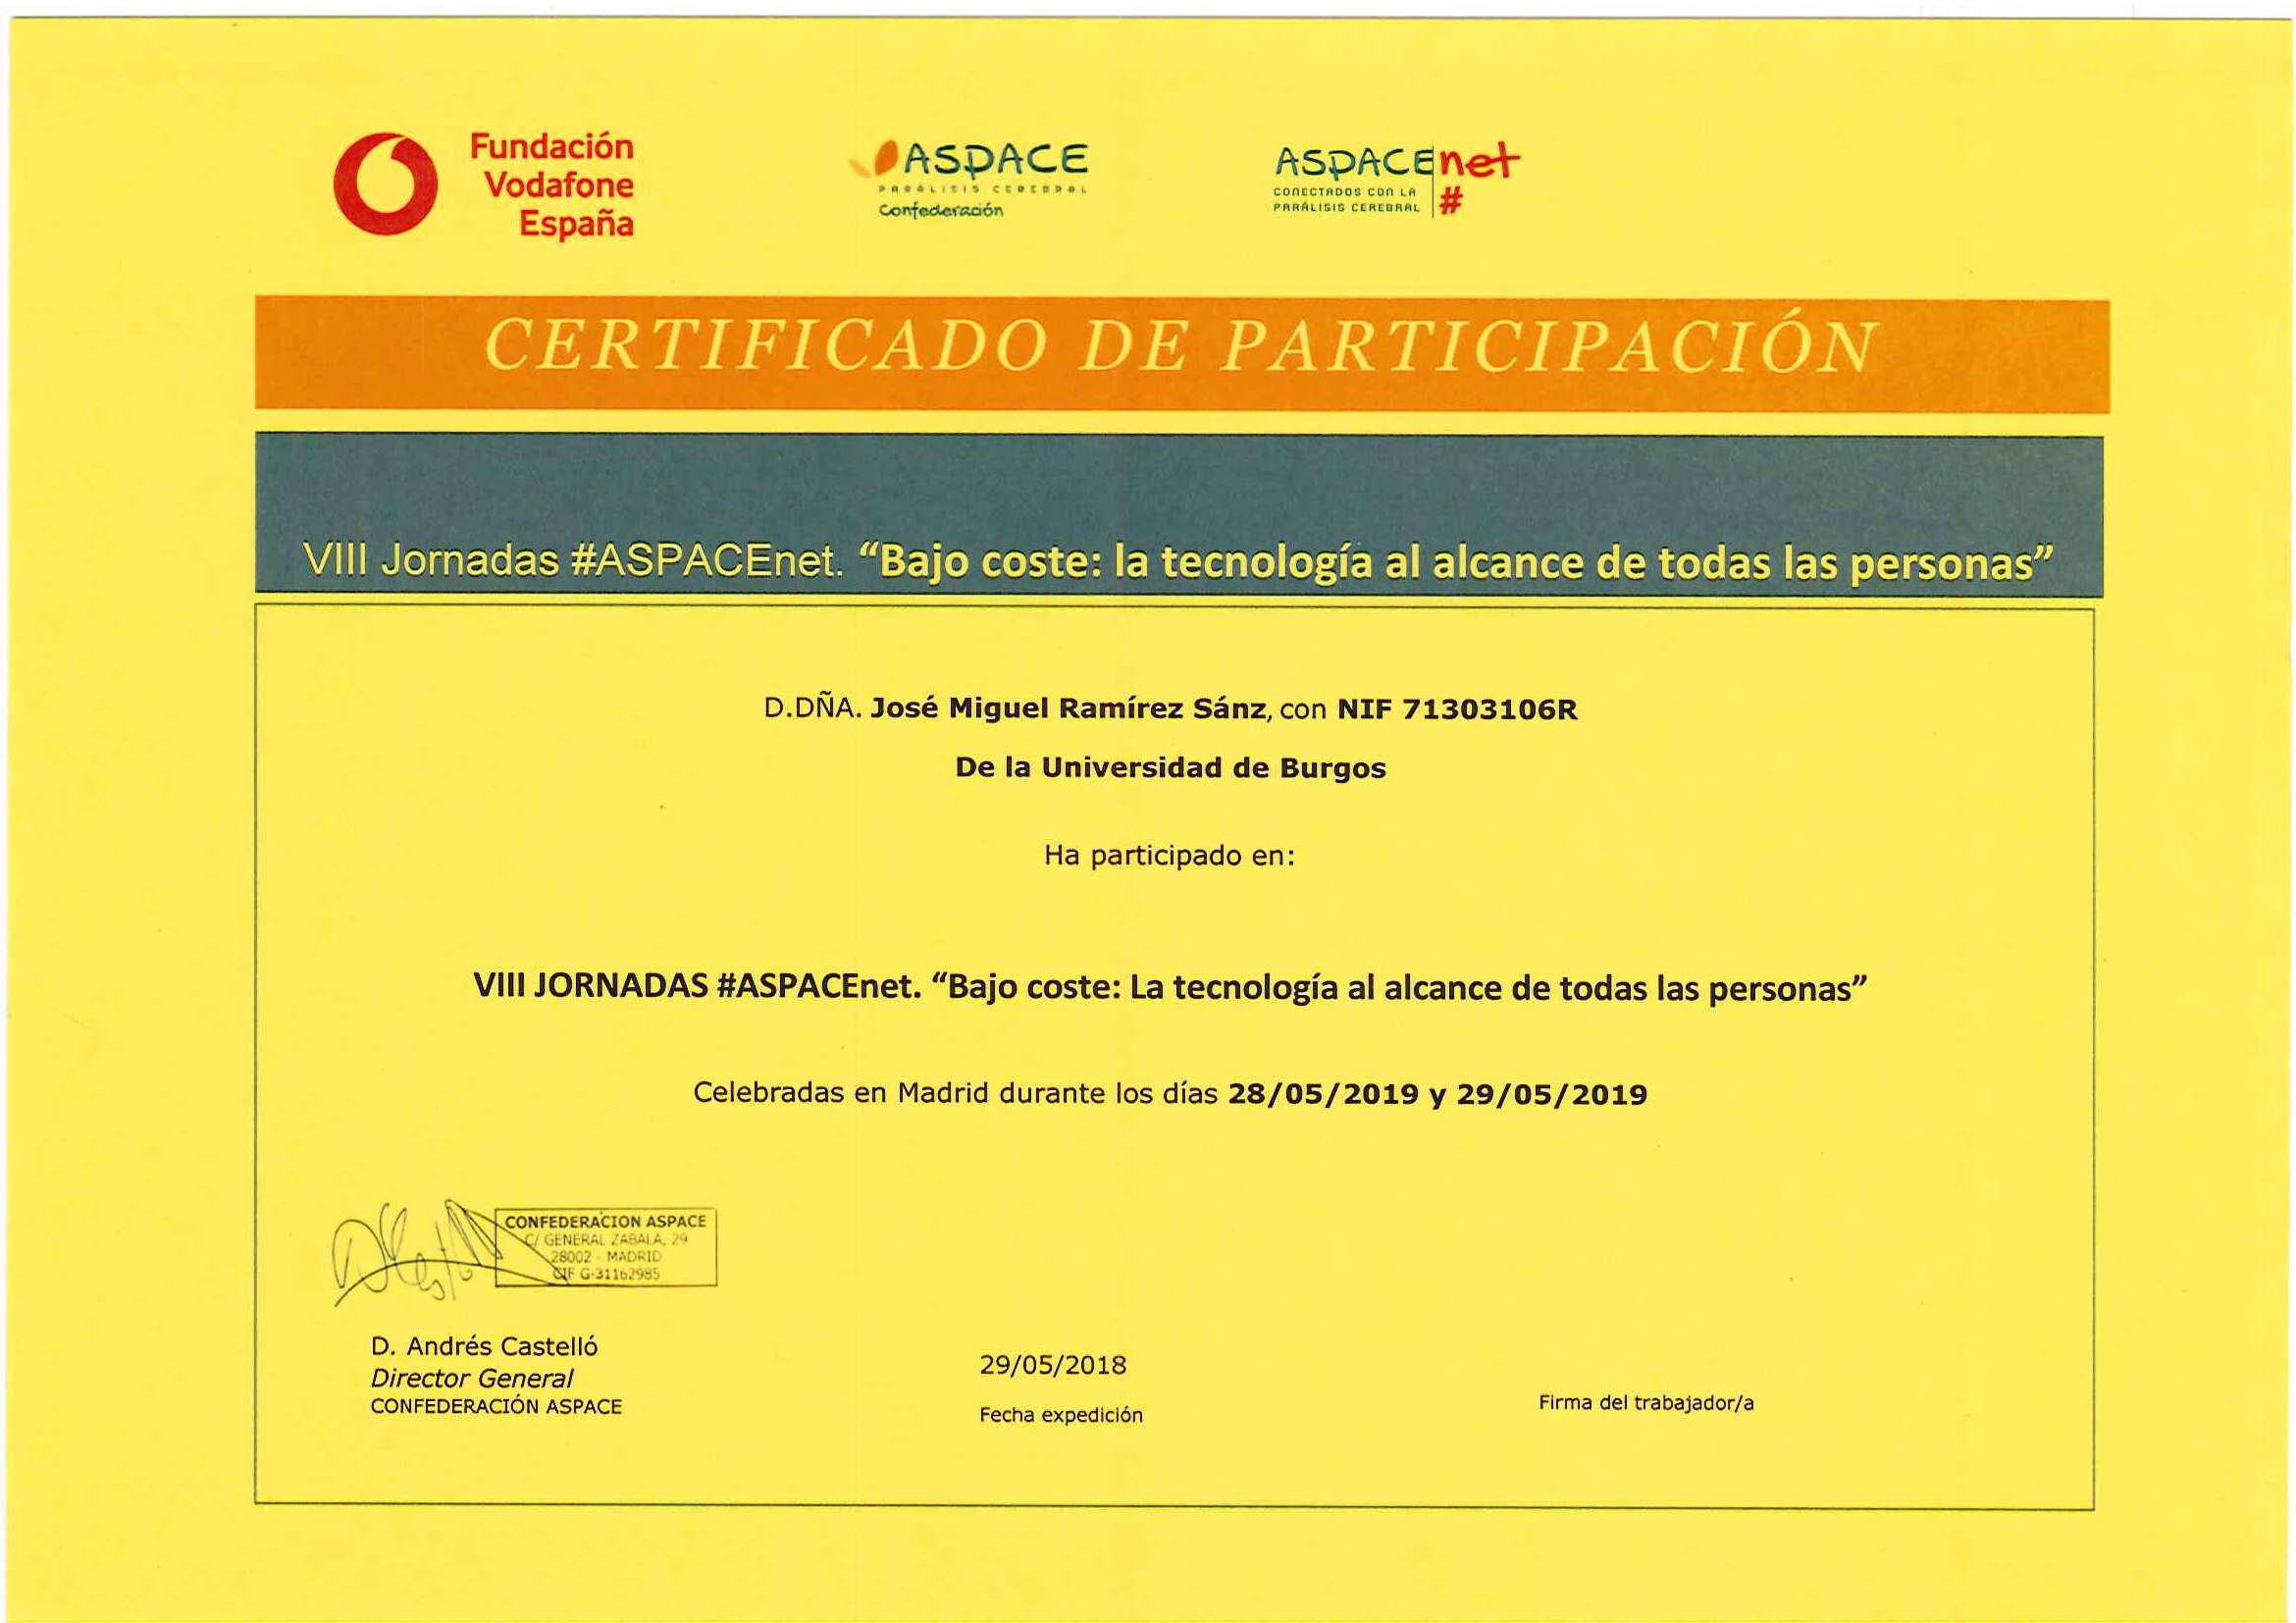
\includegraphics[width=\textwidth]{madrid}
	\caption{Certificado de asistencia a las jornadas ASPACEnet 2019 en Madrid.}
	\label{fig:madrid}
\end{figure}

\begin{figure}
	\centering
	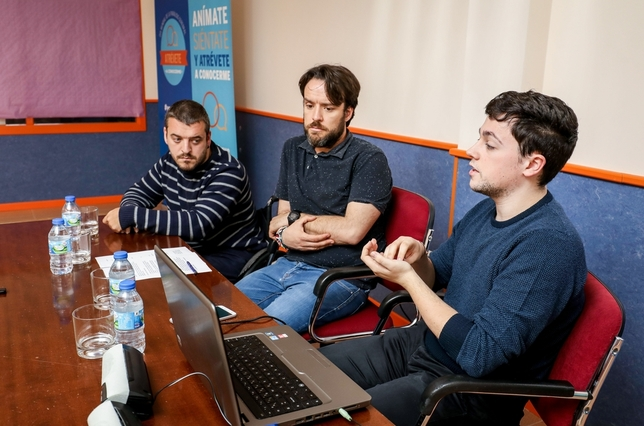
\includegraphics[width=\textwidth]{presentacionprensa}
	\caption{Imagen de la presentación ante la prensa, fuente \textit{Diario de Burgos}.}
	\label{fig:presprensa}
\end{figure}

El proyecto ha sido galardonado con los premios de Fundación Vodafone y de Becas Prototipo.
\capitulo{6}{Trabajos relacionados}

Este apartado sería parecido a un estado del arte de una tesis o tesina. En un trabajo final grado no parece obligada su presencia, aunque se puede dejar a juicio del tutor el incluir un pequeño resumen comentado de los trabajos y proyectos ya realizados en el campo del proyecto en curso. 

\capitulo{7}{Conclusiones y Líneas de trabajo futuras}

En este apartado se va comentar las conclusiones del proyecto, además de una explicación sobre las mejoras que se podrían realizar sobre éste.

\section{Conclusiones}
El proyecto merece la pena porque permite comunicarse con personas gravemente afectadas  que sin este no podrían, sobre todo en los aspectos más relevantes que son la interpretación de emociones negativas que nos permiten saber cuando le ocurre algo malo al paciente, que por desgracia, no nos lo puede decir por su propia voz.

El proyecto ha sido complicado, personalmente el proyecto más costoso en cuanto a tiempo requerido que he hecho, pero tanto desde el equipo de desarrollo de la Universidad de Burgos como desde APACE Burgos estamos contentos con el desenlace de este.

En primer lugar porque hemos cumplido todos los objetivos que nos habíamos propuesto al comienzo del proyecto. Al menos todos los objetivos que se ven mostrados en este documento, es decir, los objetivos que dependían directamente de mi trabajo. 

Como comento en el siguiente apartado en las posibles líneas futuras del trabajo, algo que me hubiera gustado probar es el funcionamiento de la aplicación de interpretación con datos de pacientes reales, pero no dependía de nosotros el poder generar los datos suficientes y tampoco se podía forzar a los pacientes a hacer esos sonidos, principalmente porque las emociones con las que hemos trabajado son negativas, ya que tanto de APACE como desde la universidad nos parecían más importantes de interpretar.

En segundo lugar, hemos podido durante todo el proyecto contar con un punto muy importante, las opiniones de los usuarios finales, es decir, opiniones de padres y madres, de los cuidadores, de los compañeros... Esta es la opinión que realmente nos interesaba. Tanto en las presentaciones a usuarios de la aplicación de generación de datos, como las presentaciones de laa aplicación de interpretación he obtenido muy buenas críticas, sobre todo en los apartados hacia los que enfocamos el proyecto, la simplicidad y la accesibilidad.

\section{Líneas de trabajo futuras}
Como ya he comentado en el apartado anterior, he cumplido casi todos los objetivos que tenía en este proyecto, aun así siempre hay puntos donde se puede mejorar. Algunas de estas mejoras son:
\begin{itemize}
	\item Uso de otro tipo de clase para la grabación en \textit{Android}, aunque \textit{MediaRecorder} no me ha dado malos resultados, siempre es mejor usar un grabación sin pérdidas.
	\item Poder tener más datos con los que poder realmente hacer un estudio de la clasificación real.
	\item Poder incluir otro clasificador que nos permita identificar el paciente a partir del audio si tener que ser seleccionado a mano.
	\item Mejorar el aspecto visual de la aplicación de generación de datos para que tenga una mayor accesibilidad.
	\item Poder realizar un estudio, con los datos suficientes, para saber si se puede generalizar el problema y así no tener que hacer un clasificador por cada paciente.
	\item Poder modificar la aplicación para que se asocie a un paciente y grabe siempre que este emite algún sonido. 
	\item Poder usar la aplicación con personas con otras discapacidad y/o enfermedades.
	\item Poder realizar una aplicación web para poder añadir y eliminar pacientes.
\end{itemize}



\bibliographystyle{plain}
\bibliography{bibliografia}

\end{document}
